\documentclass[aspectratio=169]{beamer}
\usepackage[x11names]{xcolor}


\usetheme{ucl}

%%% Increase the height of the banner: the argument is a scale factor >=1.0
% \setbeamertemplate{banner}[ucl][1.5]

%%% Change the colour of the main banner
%%% The background should be one of the UCL colours (except pink or white):
%%%   black,darkpurple,darkred,darkblue,darkgreen,darkbrown,richred,midred,
%%%   navyblue,midgreen,darkgrey,orange,brightblue,brightgreen,lightgrey,
%%%   lightpurple,yellow,lightblue,lightgreen,stone
\setbeamercolor{banner}{bg=orange}
%\setbeamercolor{banner}{bg=orange,fg=black}

%%% Add a stripe behind the banner
%\setbeamercolor{banner stripe}{bg=brightblue,fg=black}

%%% The main structural elements
% \setbeamercolor{structure}{fg=black}

%%% Author/Title/Date and slide number in the footline
\setbeamertemplate{footline}[author title date]

%%% Puts the section/subsection in the headline
%\setbeamertemplate{headline}[section]

%%% Puts a navigation bar on top of the banner
%%% For this to work correctly, the each \section command needs to be
%%% followed by a \subsection. Requires one extra compile.
% \setbeamertemplate{headline}[miniframes]
%%% Accepts an optional argument determining the width
% \setbeamertemplate{headline}[miniframes][0.3\paperwidth]


%%% Puts the frame title in the banner
%%% Won't work correctly with the above headline templates
% \useoutertheme{ucltitlebanner}
%%% Similar to above, but smaller (and puts subtitle on same line as title)
% \useoutertheme[small]{ucltitlebanner}

%%% Gives block elements (theorems, examples) a border
% \useinnertheme{blockborder}
%%% Sets the body of block elements to be clear
% \setbeamercolor{block body}{bg=white,fg=black}

%%% Include CSML logo on title slide
\titlegraphic{
\includegraphics[width=0.16\paperwidth]{IMD}}

%%% Include IMD logo in bottom right corner of all slides
% \logo{
\includegraphics[width=0.12\paperwidth]{IMD}}

%%% Set a background colour
% \setbeamercolor{background canvas}{bg=lightgrey}

%%% Set a background image
%%% Some sample images are available from the UCL image store:
%%%   https://www.imagestore.ucl.ac.uk/home/start
% \setbeamertemplate{background canvas}{%
%   \includegraphics[width=\paperwidth]{imagename}}

\hypersetup{
  colorlinks=true,
  linkcolor=blue,
  urlcolor=blue,
  citecolor=blue
}

\useoutertheme{ucltitlebanner}

%%%%%% Some other settings that can make things look nicer
%%% Set a smaller indent for description environment
\setbeamersize{description width=2em}
%%% Remove nav symbols (and shift any logo down to corner)
\setbeamertemplate{navigation symbols}{\vspace{-2ex}}



\setbeamercolor{title}{bg=white, fg=white}

\title[NSCI0032-25/26]{NSCI0032 25/26 - Lectures}
%\author[Auth. 1 \and Auth.]{Adham Hashibon \and Author 2}
\author[A. Hashibon]{Professor Adham Hashibon}
\institute[UCL]{%
 Institute for Materials Discovery \\ %
  UCL
}
\date{1. October 2025}

\begin{document}


\begin{frame}
  \titlepage%
\end{frame}

\begin{frame}{Outline}
  \tableofcontents
\end{frame}

\section{Lecture 1  }
\subsection{1.10.2025}

%%%%%%%%%%%%%%%%%%%%%%%%%
\begin{frame}
  \frametitle{Integrated Data-Driven Materials Science and Digitalisation}
  \framesubtitle{NSCI0032 - Cohort 2025-2026 }
  \begin{itemize}
    \item Lecturer: {\bf Professor Adham Hashibon} 
      \begin{itemize}
        \item Head of the Data-Driven Materials Discovery and Informatics Group (DDMDi) 
        \item Module and AMS Programme lead 
        \item Director of the Institute for Materials Discovery 
      \end{itemize}
    \item You can contact me at: \href{mailto://a.hashibon@ucl.ac.uk}{a.hashibon@ucl.ac.uk}
    \item \href{https://moodle.ucl.ac.uk/course/view.php?id=47590}{Moodle Page - Is being rolled over - Stay Tuned! we could review it tomorrow!}
    \item \href{https://www.ucl.ac.uk/module-catalogue/modules/integrated-data-driven-materials-science-and-digitalisation-NSCI0032}{Module Catalouge}  
    \item 4 hours every week,  3 h are lectures, and 1 h hands on tutorial.
    \pause%
  \item \alert{However}, some of the lectures will be more interactive than others
  \end{itemize}
\end{frame}

\begin{frame}
  \frametitle{Overview}
%  \framesubtitle{What are we going to learn?}

  \begin{alertblock}{What are we going to learn?}
    The module “Integrated Data-Driven Materials Science and Digitalisation” provides students with state-of-the art knowledge and expertise in {\it integrated materials} modelling, methods and practical modern advanced {\it cloud-based} tools to find `and create needed materials and process {\it data} for applications in advanced data-driven and {\it machine learning} workflows. 
  \end{alertblock}

%  \begin{example}
%    \begin{itemize}
%    \item 3
%    \item 4
%    \end{itemize}
%  \end{example}
\end{frame}


\begin{frame}
  \frametitle{What are we going to learn?}
    It covers contemporary topics in 
    \begin{itemize}
      \item {\it Digitalisation} based on emerging {\it ontology} of materials and processes and connection to manufacturing ({\it digital twins})
     \item {\it High-Throughput Computations} and {\it Characterisation}
     \item {\it Multiscale}, and Multi-Equation physics based modelling, including
       \begin{itemize}
         \item Electronic density functional theory (DFT)
         \item Atomistic molecular dynamics (MD)
         \item Mesoscopic coarse-grained molecular dynamics (CGMD),
         \item continuum structural mechanics and computational fluid mechanics (CFD) modelling,
   \end{itemize}
     \item Enabling modelling technological applications on all relevant scales.
   \end{itemize}

\end{frame}



\begin{frame}{What are we going to learn?}
  \begin{columns}[T] % [T] = align columns at top
    \begin{column}{0.5\textwidth}
     Advanced modern tools include cloud-based open e-science materials digitalisation and modelling platforms such as
      \begin{itemize}
        \item \href{https://nanohub.org}{nanoHUB}
        \item \href{https://materialsproject.org}{Materials Project}
        \item \href{https://www.nomad-coe.eu/the-project/nomad-repository}{NOMAD Repository}
        \item \href{https://www.materialscloud.org/work/aiidalab}{Materials Cloud — AiiDA Lab}
%        \item \href{https://aflowlib.org}{AFLOWlib (AFLOW)}
%        \item \href{https://oqmd.org}{OQMD}
%        \item \href{https://jarvis.nist.gov}{JARVIS (NIST)}
%        \item \href{https://openkim.org}{OpenKIM}
        \item and other emerging platforms (like ours... name to be decided... )
      \end{itemize}
    \end{column}

    \begin{column}{0.5\textwidth}
      \centering
      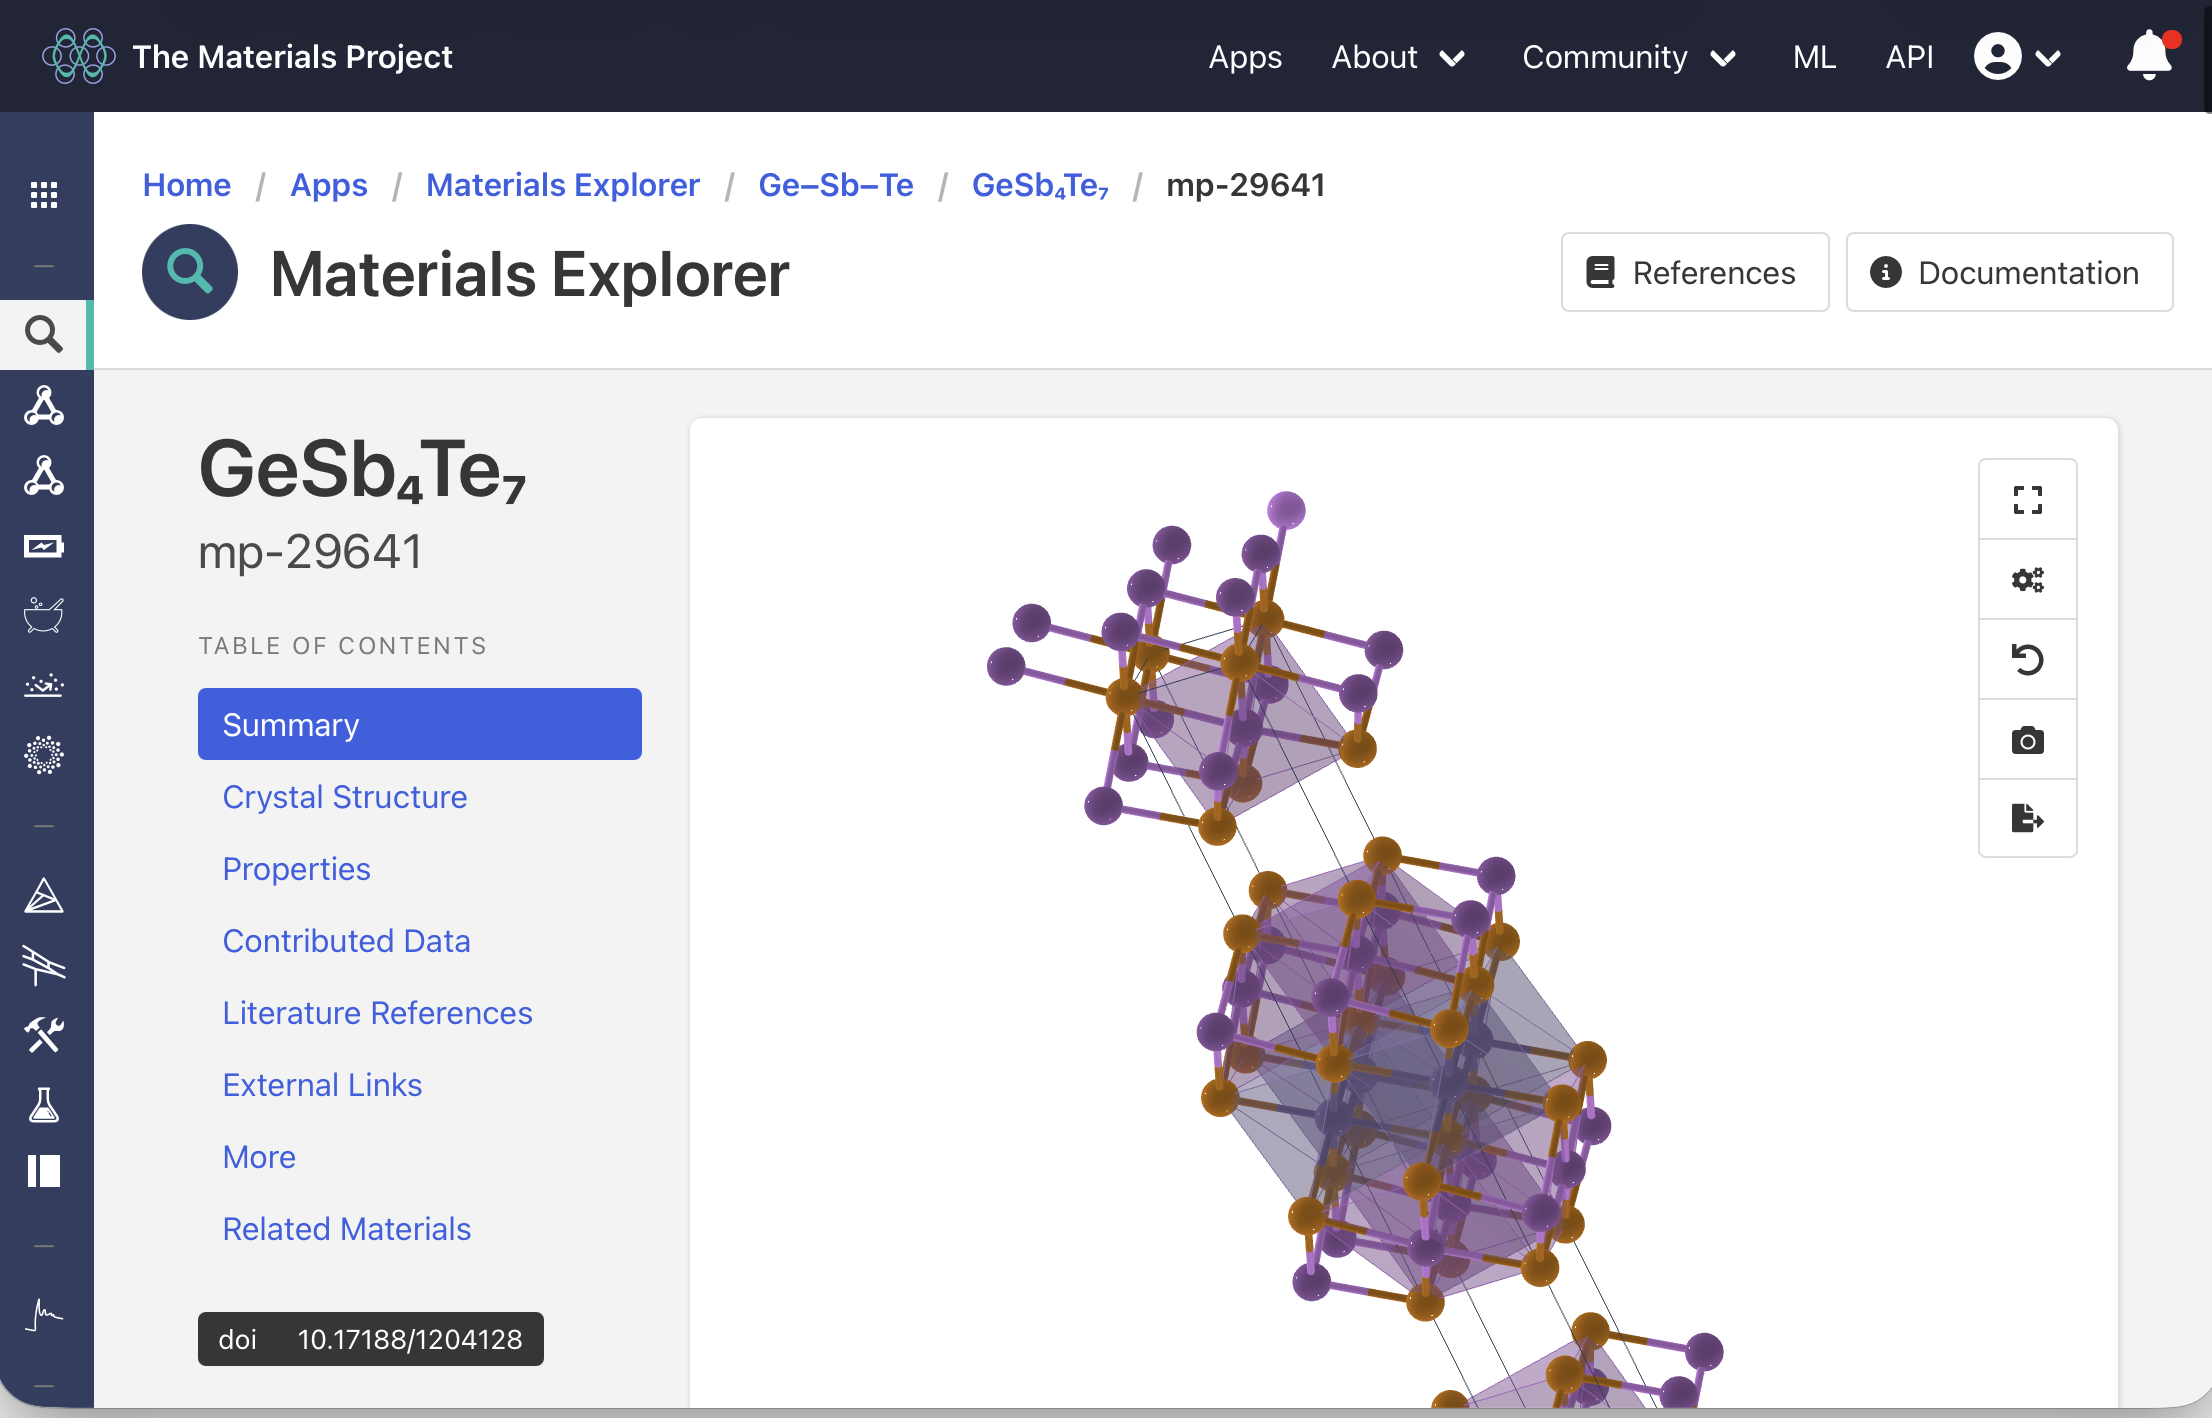
\includegraphics[width=\linewidth]{media/mp.png}
    \end{column}
  \end{columns}
\end{frame}

%%% from here on, remove branding from banners
\setbeamertemplate{banner}[blank]


\section{Lecture 2 (Teaching Week 1)}
\subsection{Thursday 2nd of October 2025}



%%% use department headline template
%\setbeamertemplate{headline}[department]

%%% set department and subdepartment
%%\setbeamertemplate{department}{Department of Sample Science}
%%\setbeamertemplate{subdepartment}{Subdepartment slogan}


%%% use footline template
%\setbeamertemplate{footline}[author title date]
%\setbeamercolor{footline}{use=banner, bg=black, fg=banner.fg!80!banner.bg}


\begin{frame}{Learning Objectives}


%%%%%%%%%%%%%%%%%%%%%%%%%%%%%%%%%%%%%%%%%%%%
\begin{itemize}
  \item Terminology and Data Science Basics
  \item Gain understanding and clarity of what data-driven science means.
  \item Understand the roles of data-based versus physics-based modelling.
  \item Learn about the exciting emerging open science platforms and how to utilise them 
\end{itemize}
\end{frame}
%%%%%%%%%%%%%%%%%%%%%%%%%%%%%%%%%%%%%%%%%%%%


%%%%%%%%%%%%%%%%%%%%%%%%%%%%%%%%%%%%%%%%%%%%
\begin{frame}{Learning Outcomes}
 \begin{itemize}
   \item Terminology and Data Science Basics
  \item Clear overview of the data-driven materials discovery field.
  \item Types of modelling.
  \item Bird's eye view of materials discovery.
  \item Understand what we want to achieve in this module and how to find additional relevant information.
  \item Learn about existing infrastructure and tools.
\end{itemize} 
\end{frame}
%%%%%%%%%%%%%%%%%%%%%%%%%%%%%%%%%%%%%%%%%%%%


%%%%%%%%%%%%%%%%%%%%%%%%%%%%%%%%%%%%%%%%%%%%
\begin{frame}{Integrated Data-Driven Materials Science and Digitalisation}
  \begin{itemize}
    \item Integrated
    \item Data Driven
    \item Materials Science
    \item Digitalisation
    \item \dots
  \end{itemize}
\end{frame}
%%%%%%%%%%%%%%%%%%%%%%%%%%%%%%%%%%%%%%%%%%%%


%%%%%%%%%%%%%%%%%%%%%%%%%%%%%%%%%%%%%%%%%%%%
\begin{frame}{Materials and Materials Science \& Engineering}
  \begin{itemize}
    \item Materials are almost anything we study.
    \item Materials Science \& Engineering is about understanding the properties, processing and performance, and design of human-made materials (artefacts).
  \end{itemize}
\end{frame}
%%%%%%%%%%%%%%%%%%%%%%%%%%%%%%%%%%%%%%%%%%%%

%%%%%%%%%%%%%%%%%%%%%%%%%%%%%%
\begin{frame}{Examples}
  \begin{itemize}
    \item Steels, metals, alloys
    \item Semiconductors
    \item Concrete, ceramics
    \item Battery materials, neuromorphic, soft matter
    \item Synthesis and processing, \dots
    \item Mechanical, thermal properties, corrosion
    \item Electronic structure
  \end{itemize}
\end{frame}
%%%%%%%%%%%%%%%%%%%%%%%%%%%%%%


%%%%%%%%%%%%%%%%%%%%%%%%%%%%%%
\begin{frame}{Human-Made Materials vs. Life on Earth}
   \begin{columns}[T]
    \begin{column}{0.58\textwidth}
      \begin{itemize}
        \item Human-made materials now equal the weight of all life on Earth.
        \item Rapid growth in concrete, asphalt, metal, and plastic.
        \item 2020 may mark the tipping point where artificial materials outweigh living things.
        \item Study highlights the literal massiveness of humanity's planetary footprint.
      \end{itemize}
      \vfill
     {\tiny Sources:
  Scientific American, \textit{Human-Made Stuff Now Outweighs All Life on Earth}, \href{https://www.scientificamerican.com/article/human-made-stuff-now-outweighs-all-life-on-earth/}{scientificamerican.com} \\
  National Geographic, \textit{Human-made materials now equal weight of all life on Earth}, \href{https://www.nationalgeographic.com/environment/article/human-made-materials-now-equal-weight-of-all-life-on-earth}{nationalgeographic.com}
  }
    \end{column}
    \begin{column}{0.42\textwidth}
     \centering
     \begin{minipage}[t]{0.4\textwidth}
       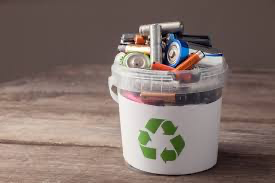
\includegraphics[height=2cm]{media/bat_recycle.png}
       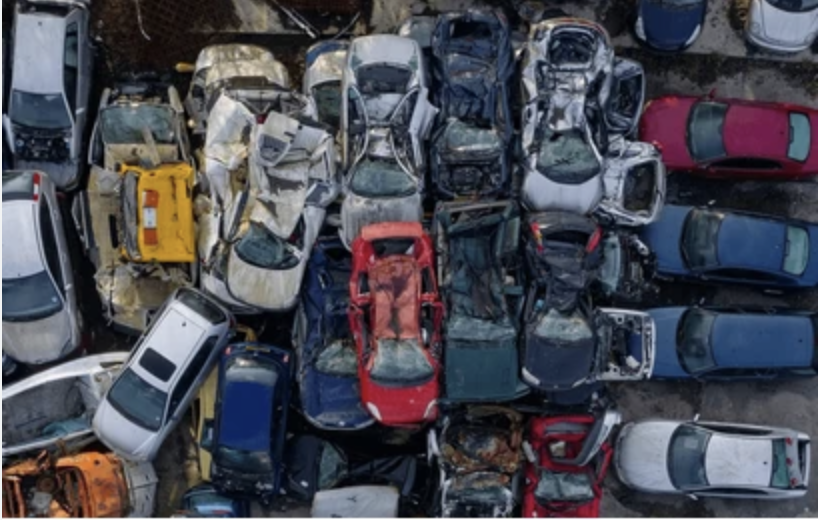
\includegraphics[width=3cm]{media/car_scrap.png}
       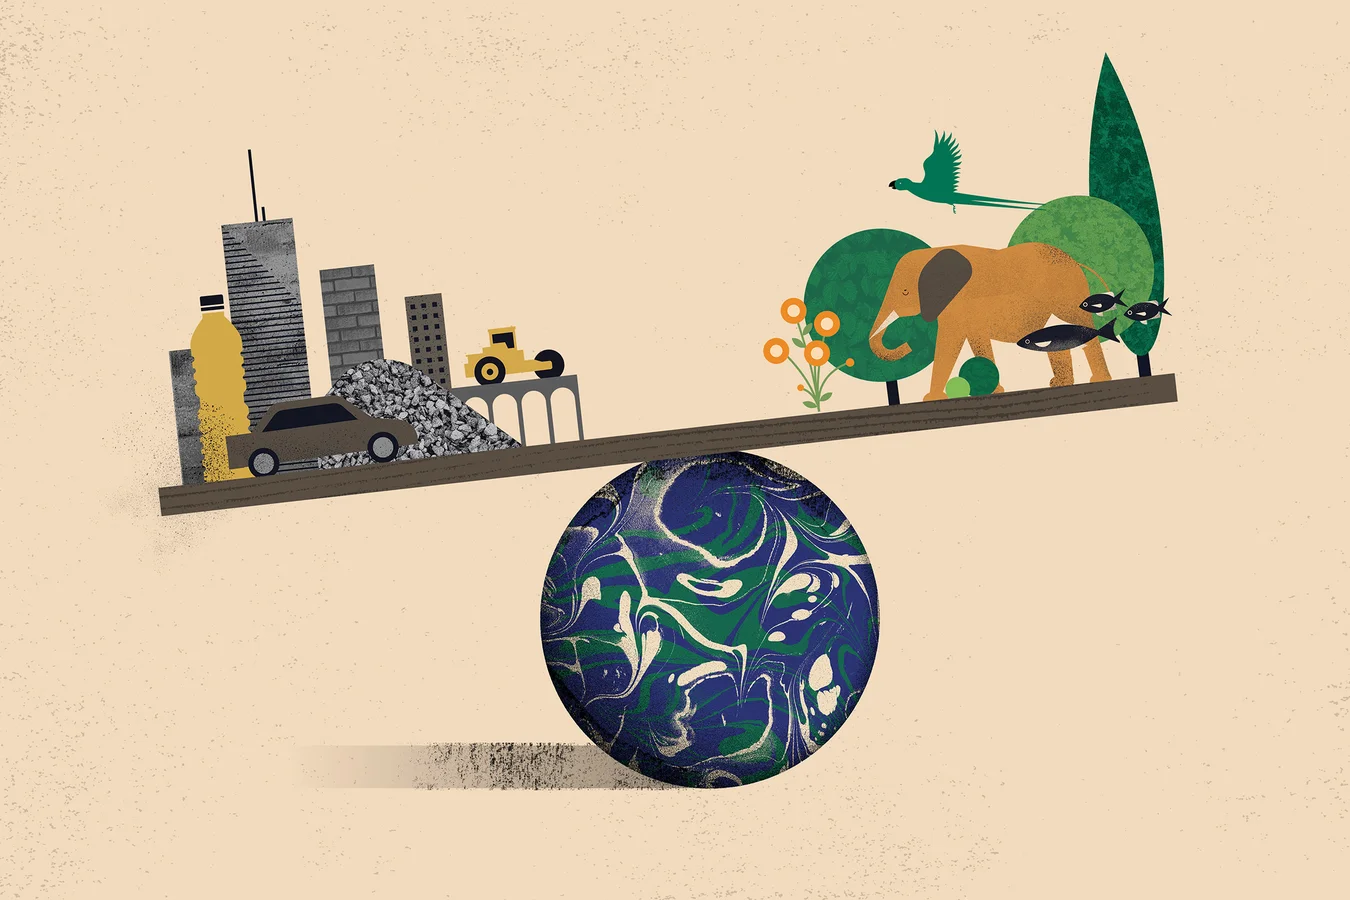
\includegraphics[width=4cm]{media/bio_versus_artifact_mass_balance.png}
     \end{minipage}
    \end{column}

   \end{columns}
\end{frame}
%%%%%%%%%%%%%%%%%%%%%%%%%%%%%%

%%%%%%%%%%%%%%%%%%%%%%%%%%%%%%
\begin{frame}{Did You Know}
  \begin{columns}
    \begin{column}{0.7\textwidth}
      \begin{itemize}
        \item Neuromorphic computing is inspired by the structure and function of the human brain.
        \item Schematics show memristive switching by filament formation and rupture (top) or phase change (bottom).
        \item The way the filament changes phase in response to stimuli could offer a pathway for "learning".
        \item This behavior is comparable to the axon in a biological neuron.
        \item The Intel Loihi uses neuromorphic computing principles, yet relies on traditional metal-oxide semiconductors.
      \end{itemize}
    \end{column}
    \begin{column}{0.3\textwidth}
     \begin{minipage}[t]{0.4\textwidth}
       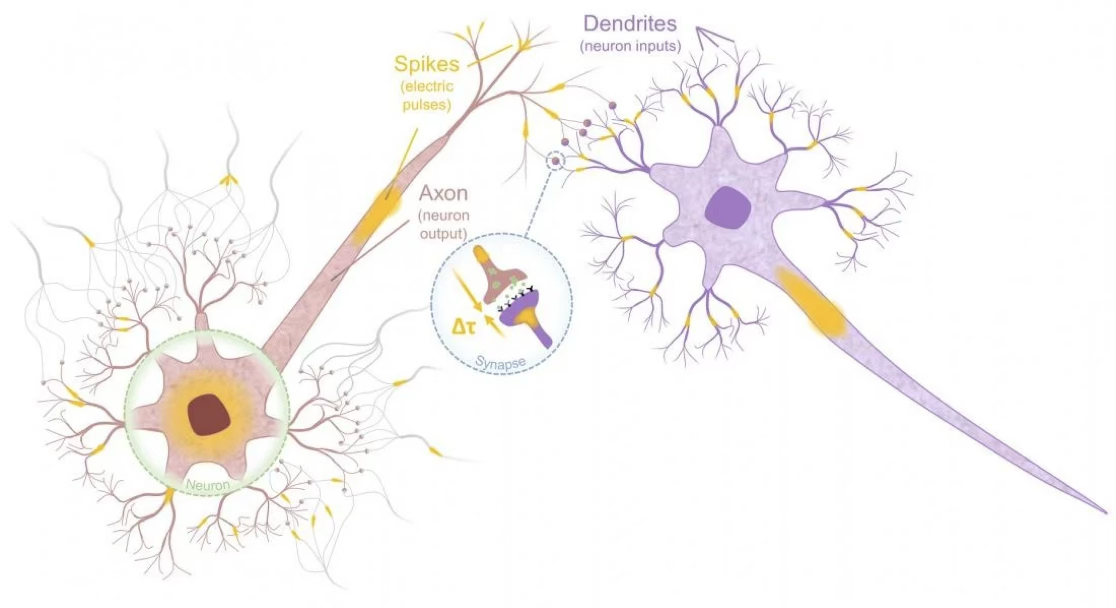
\includegraphics[width=4cm]{media/neuron.png}
       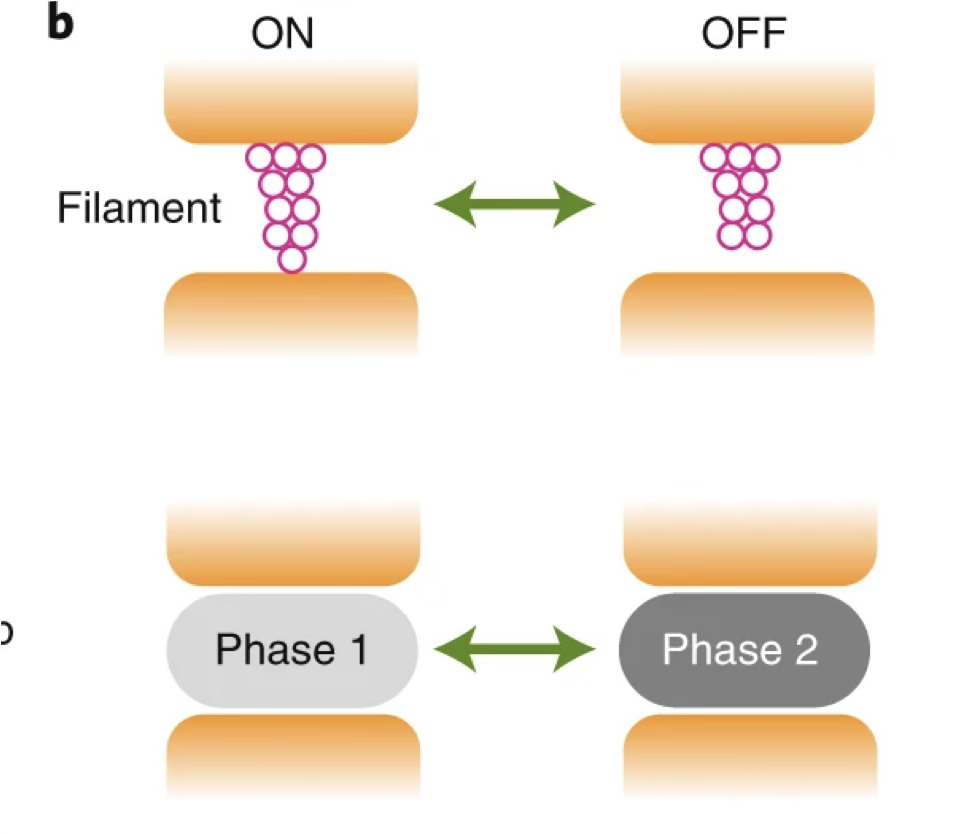
\includegraphics[width=4cm]{media/memristor.png}
       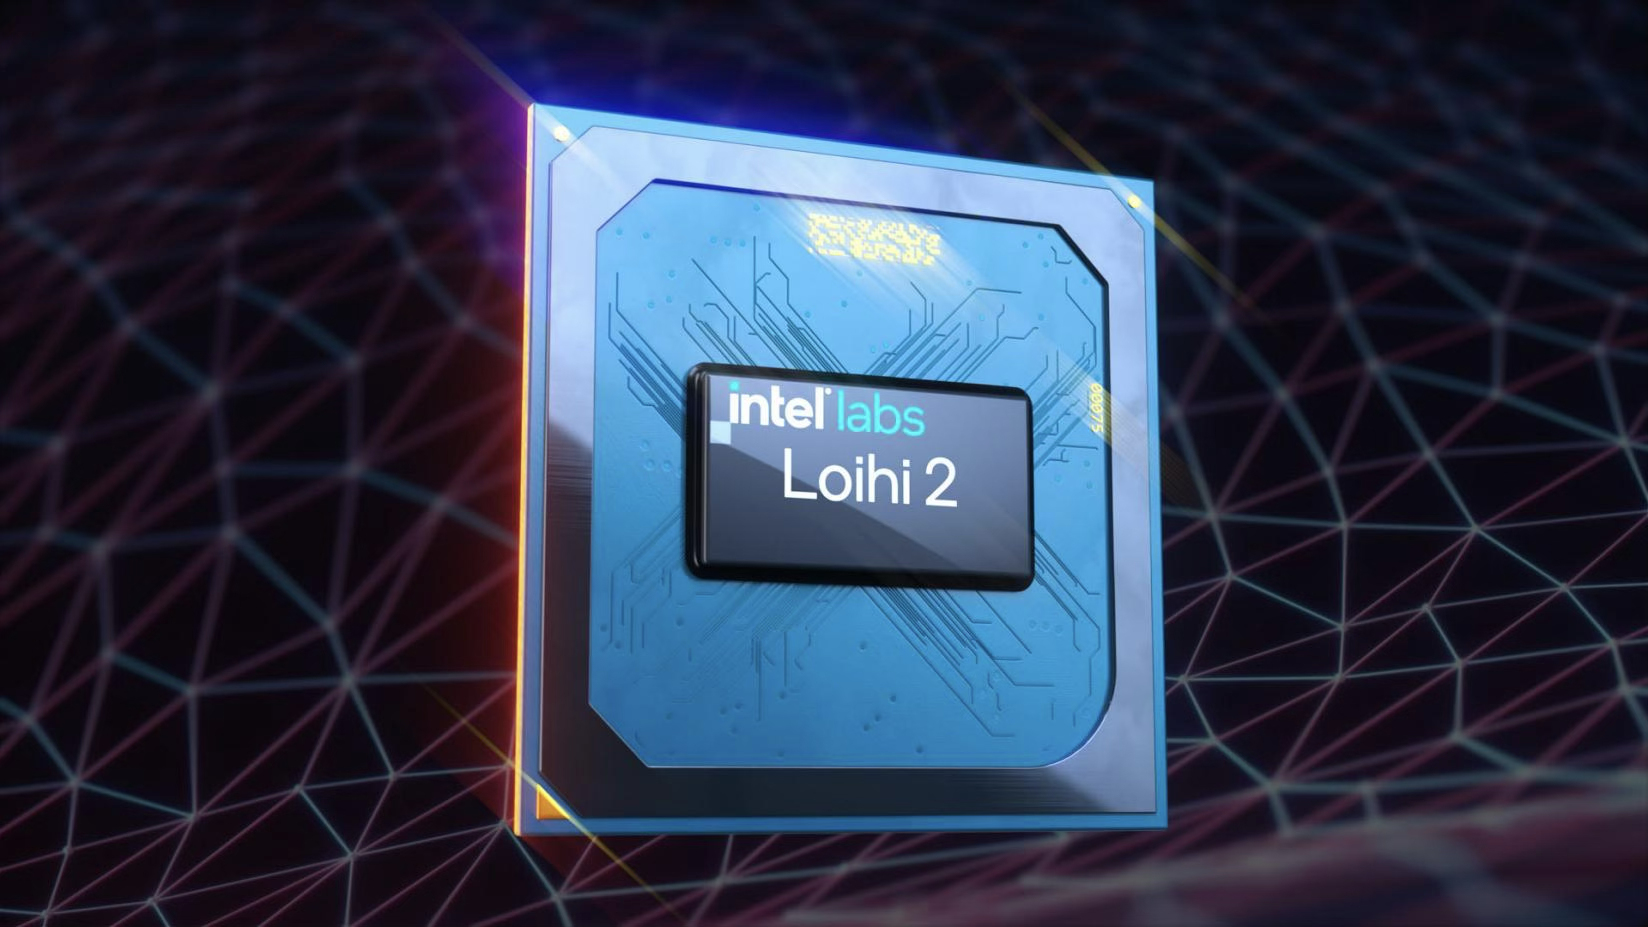
\includegraphics[width=1cm]{media/loihi2.png}
     \end{minipage}
    \end{column}
  \end{columns}
\end{frame}
%%%%%%%%%%%%%%%%%%%%%%%%%%%%%%


\begin{frame}{Neuromorphic Materials: Chalcogenides}
  \begin{columns}
    \begin{column}{0.6\textwidth}
      \begin{itemize}
        \item \textbf{Chalcogenides} are a class of phase-change materials (PCMs) 
        \item Can reversibly switch between an \textit{amorphous (glassy)} phase and a \textit{crystalline} phase, triggered by thermal energy or electric fields.
        \item This switching enables \textbf{non-volatile memory} (e.g., PC-RAM), which retains data without power.
        \item \textbf{Computational materials modelling} helps study their atomistic and electronic behavior:
        \begin{itemize}
          \item Phase transitions and energy barriers
          \item Thermodynamic stability and mechanical properties
          \item Thermal and electronic transport
        \end{itemize}
        \item Crystalline phases often contain defects: point defects, dislocations, and impurities.
      \end{itemize}
    \end{column}
    \begin{column}{0.4\textwidth}
      \centering
      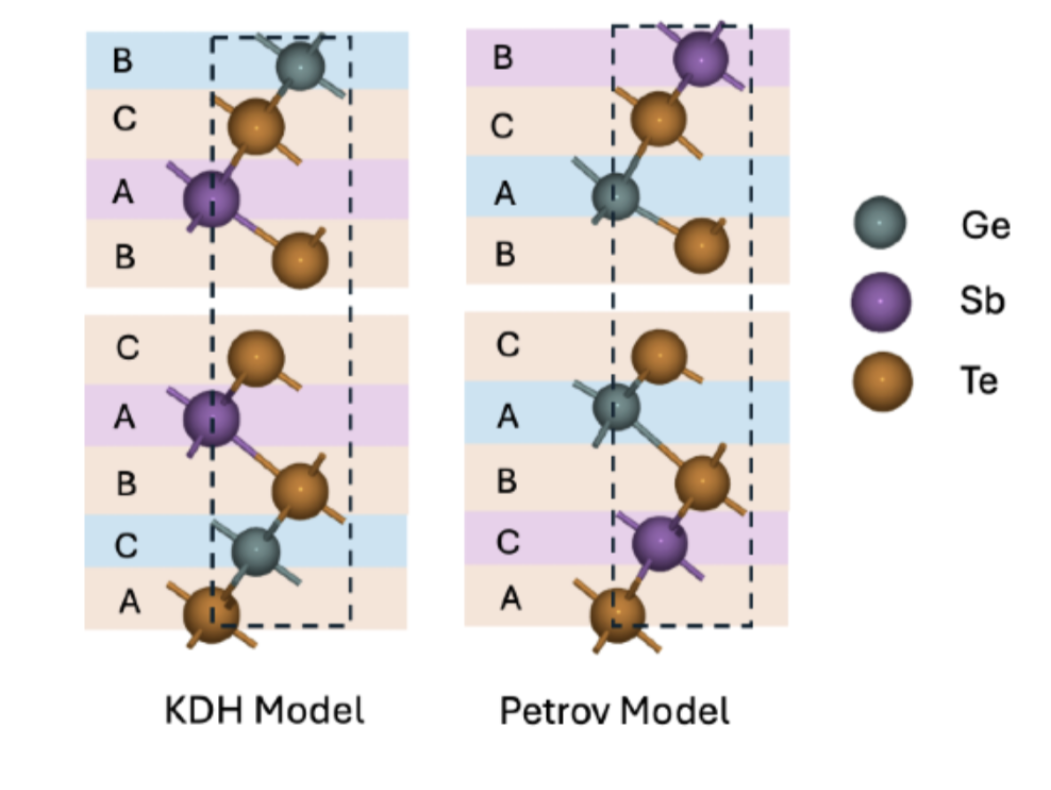
\includegraphics[height=0.3\textheight]{media/gst_models.png}
      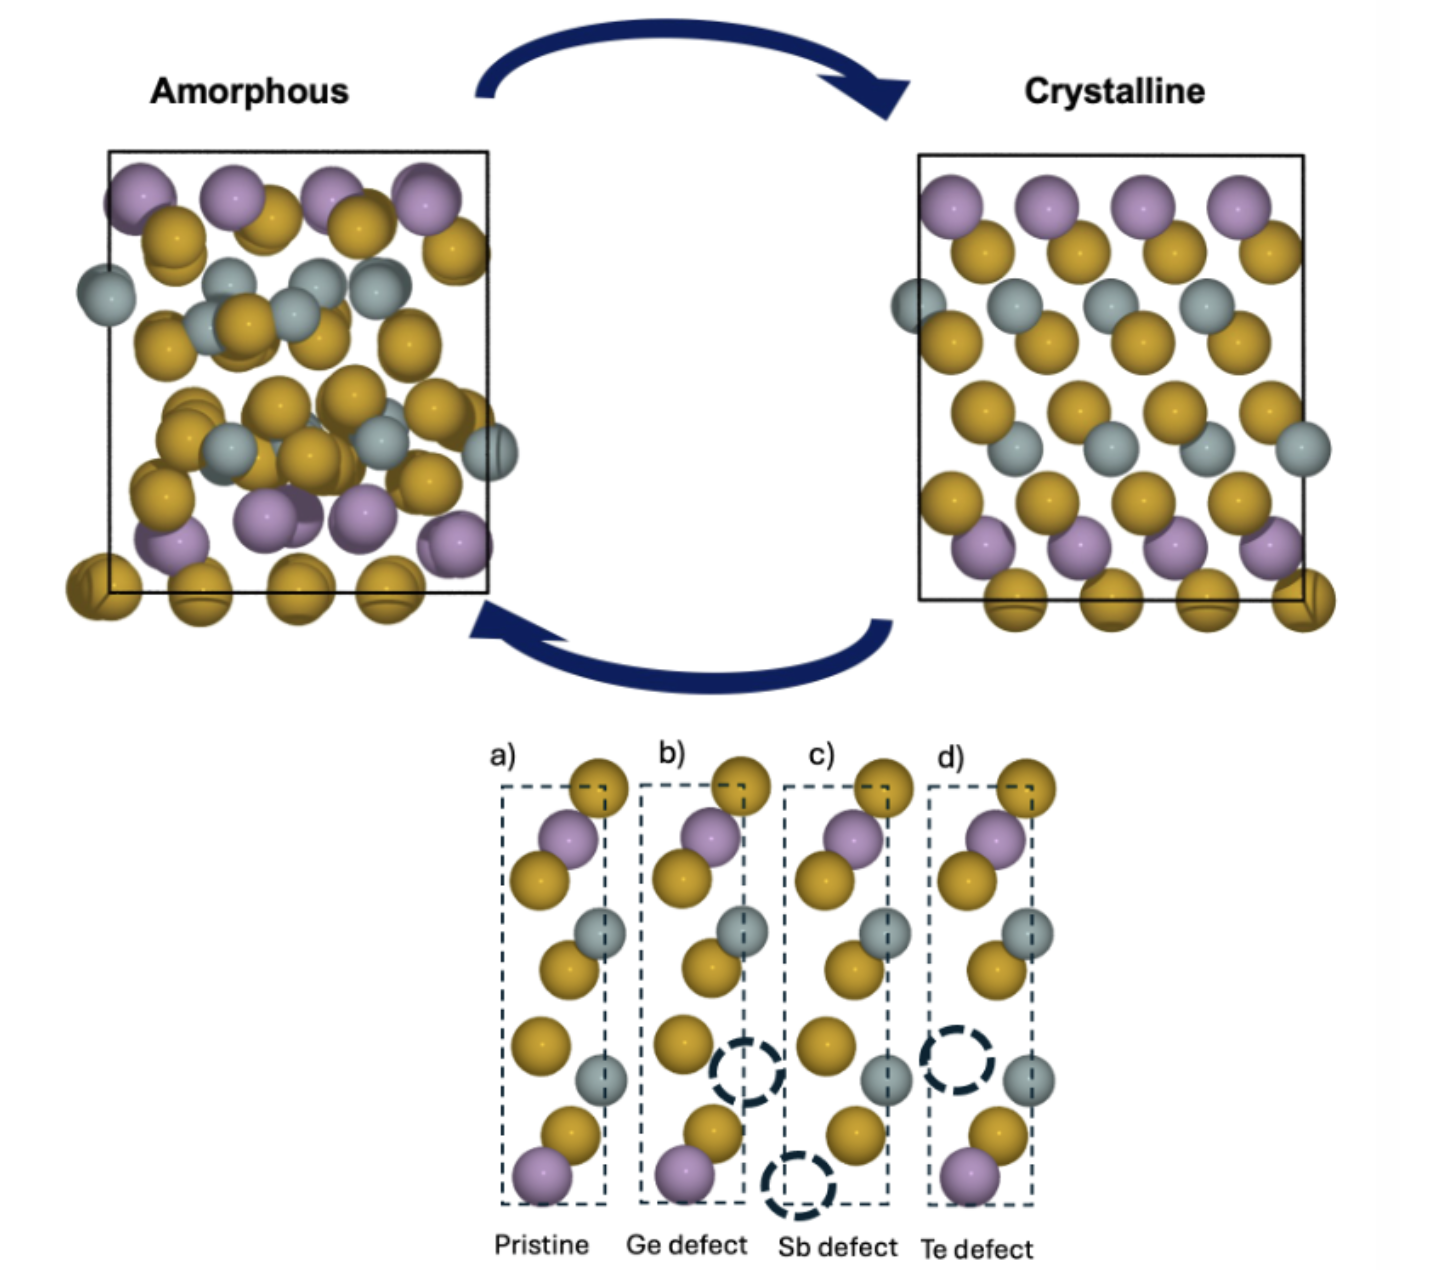
\includegraphics[height=0.4\textheight]{media/gst_phases.png}
    \end{column}
  \end{columns}
\end{frame}





\begin{frame}{Point Defects in Crystals}
  \begin{columns}
    \begin{column}{0.65\textwidth}
      \small
      \begin{itemize}
        \item Crystals are not perfect, they contain various types of defects! 
        \item The simplest defects are {\bf Point defects}:
        \begin{itemize}
          \item \textbf{Vacancies}: Missing atoms 
          \item \textbf{Self-interstitials}: Extra atoms squeezed into the lattice
          \item \textbf{Interstitial impurities}: Foreign atoms occupying spaces between lattice sites
          \item \textbf{Substitutional impurities}: Foreign atoms replacing host atoms
        \end{itemize}
        \item These defects affect electronic transport, thermal conductivity, and phase stability
      \end{itemize}
    \end{column}
    \begin{column}{0.40\textwidth}
      \centering
      \vfill
      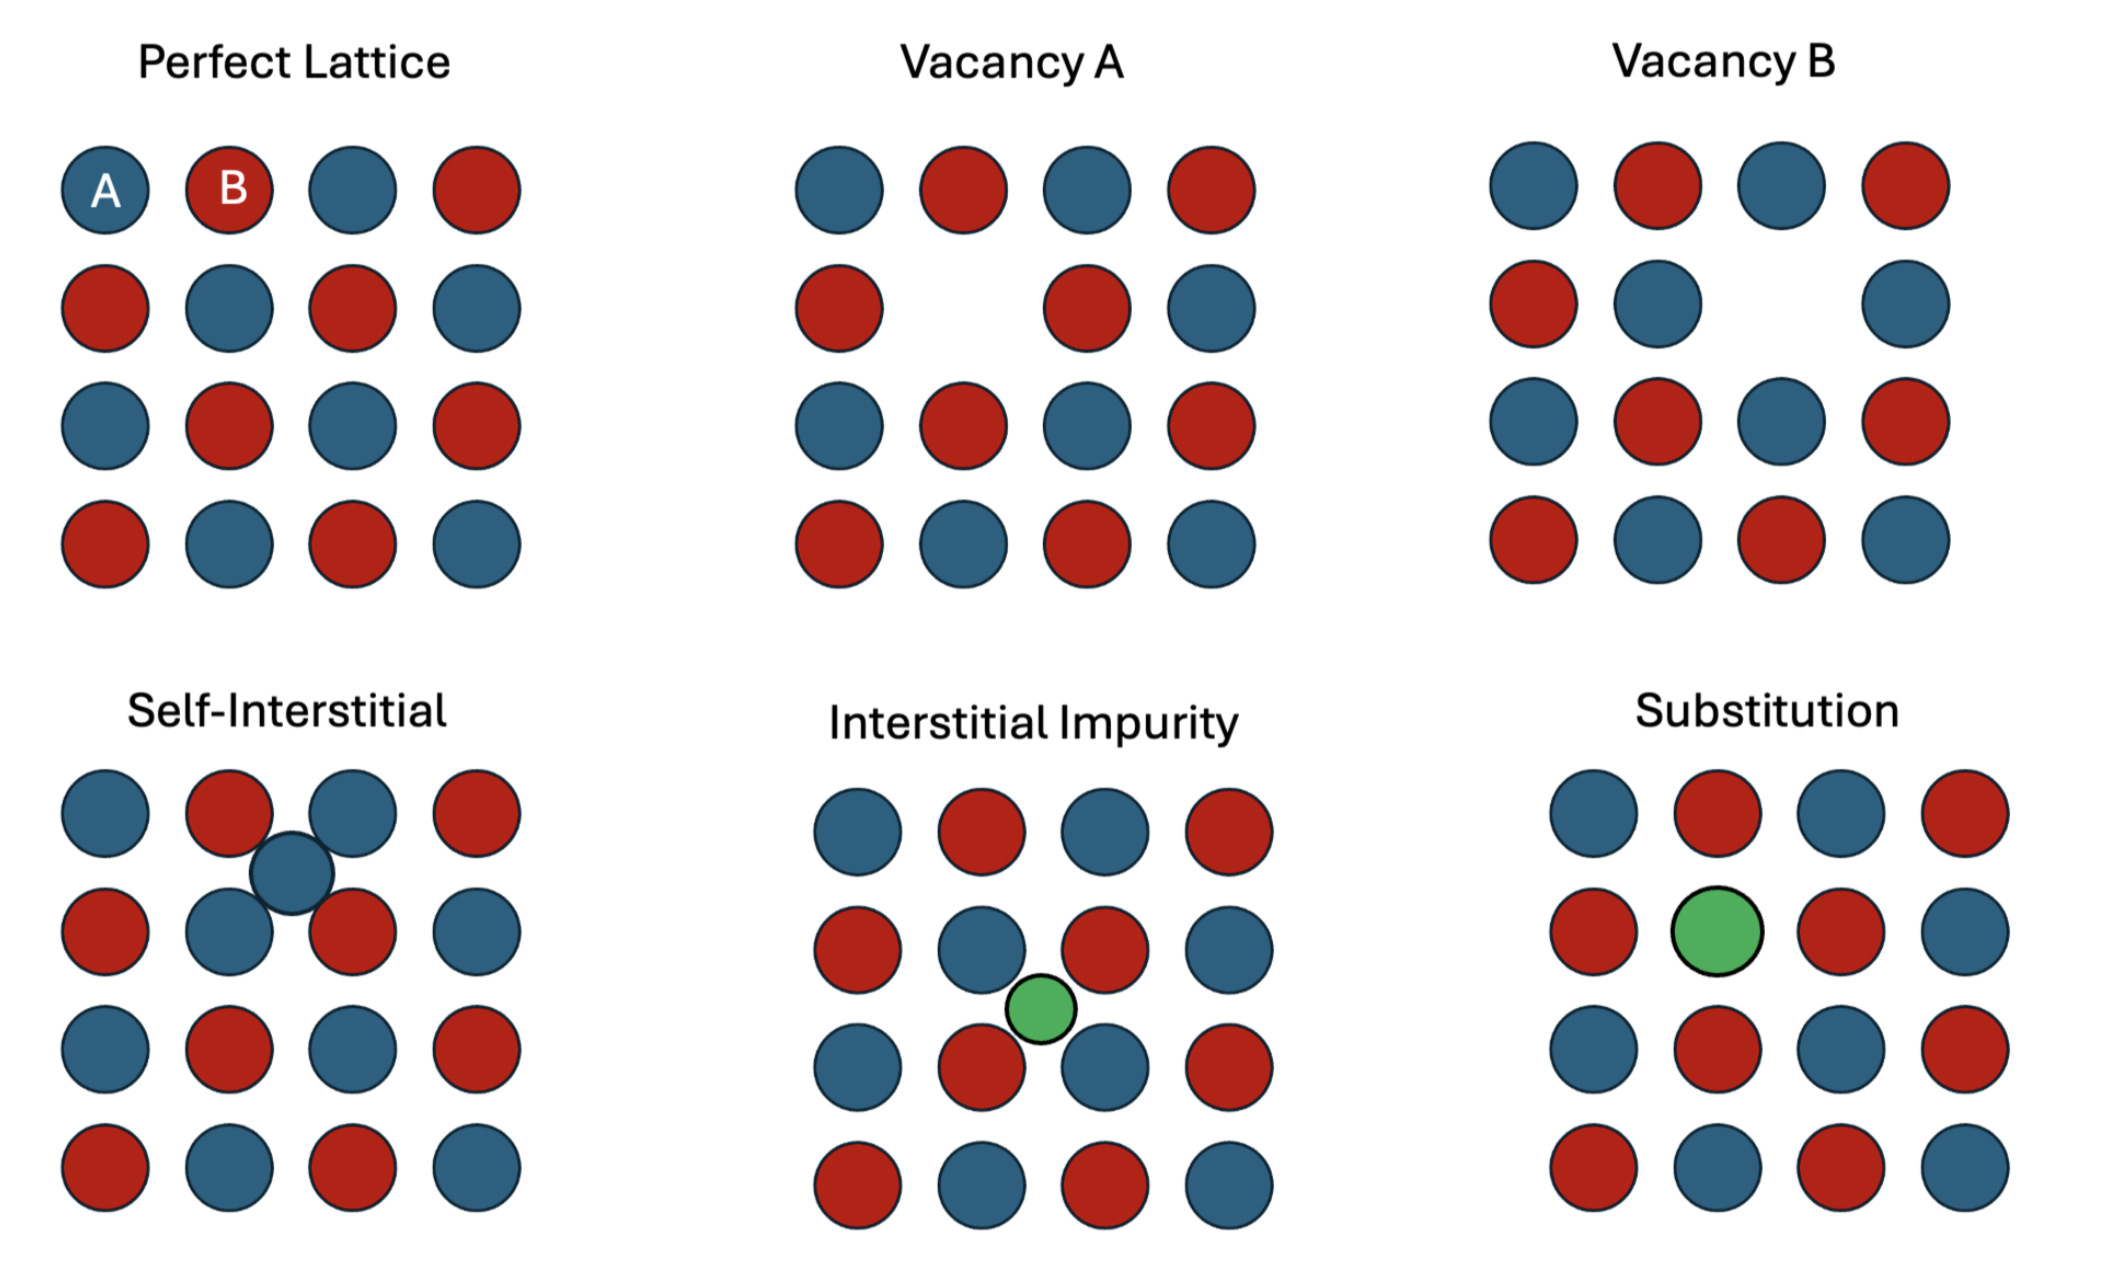
\includegraphics[width=\textwidth]{media/point_defects.png}
      \vfill
    \end{column}
  \end{columns}
\end{frame}


\begin{frame}{Example of DFT calculation}
  \centering
  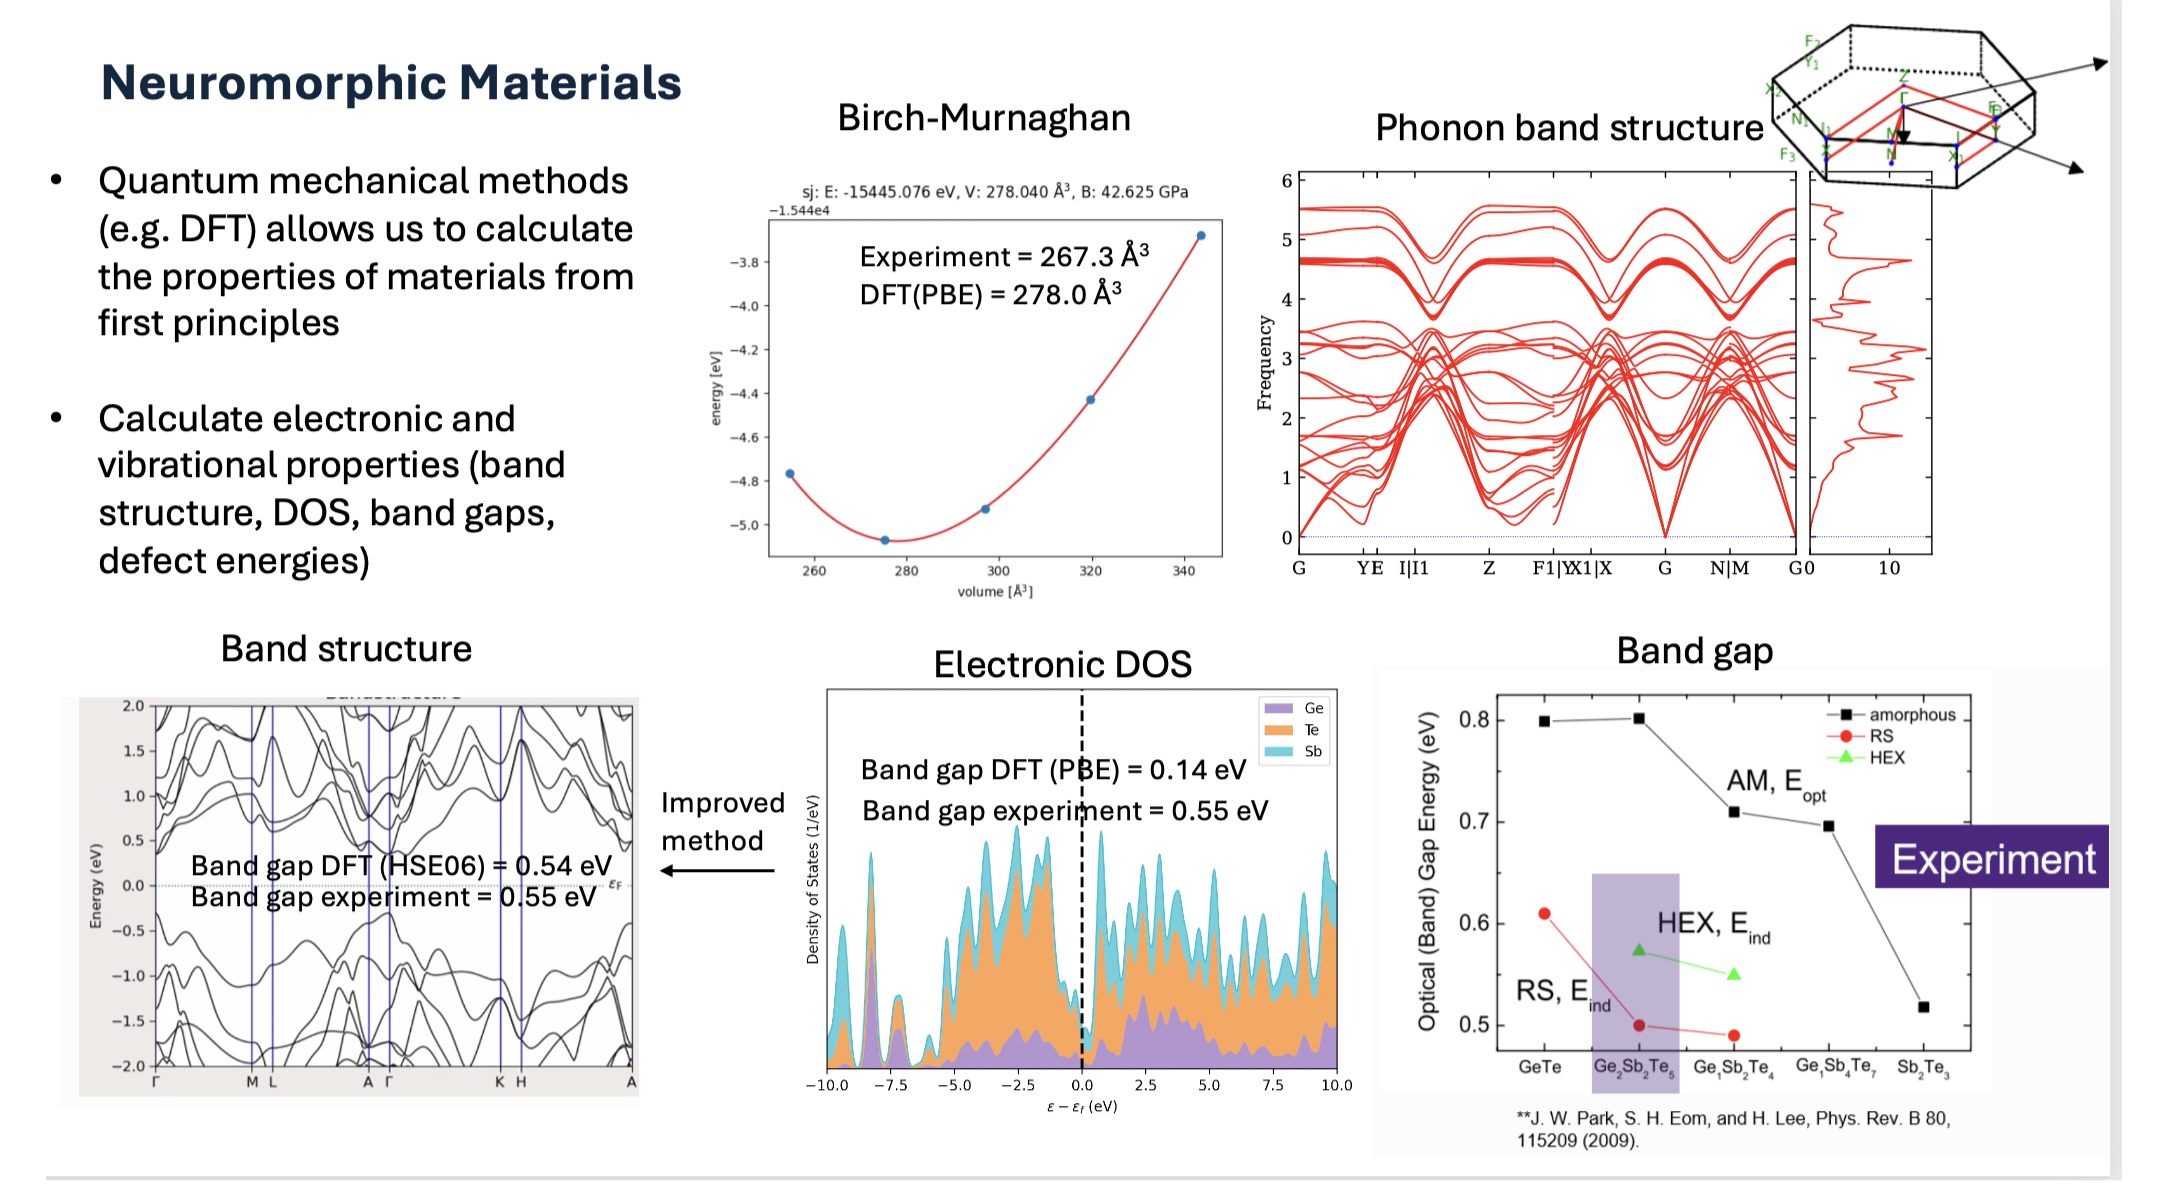
\includegraphics[width=0.75\textwidth]{media/GST_DFT.png}
\end{frame}


\begin{frame}{Example of MD calculation}
  \centering
  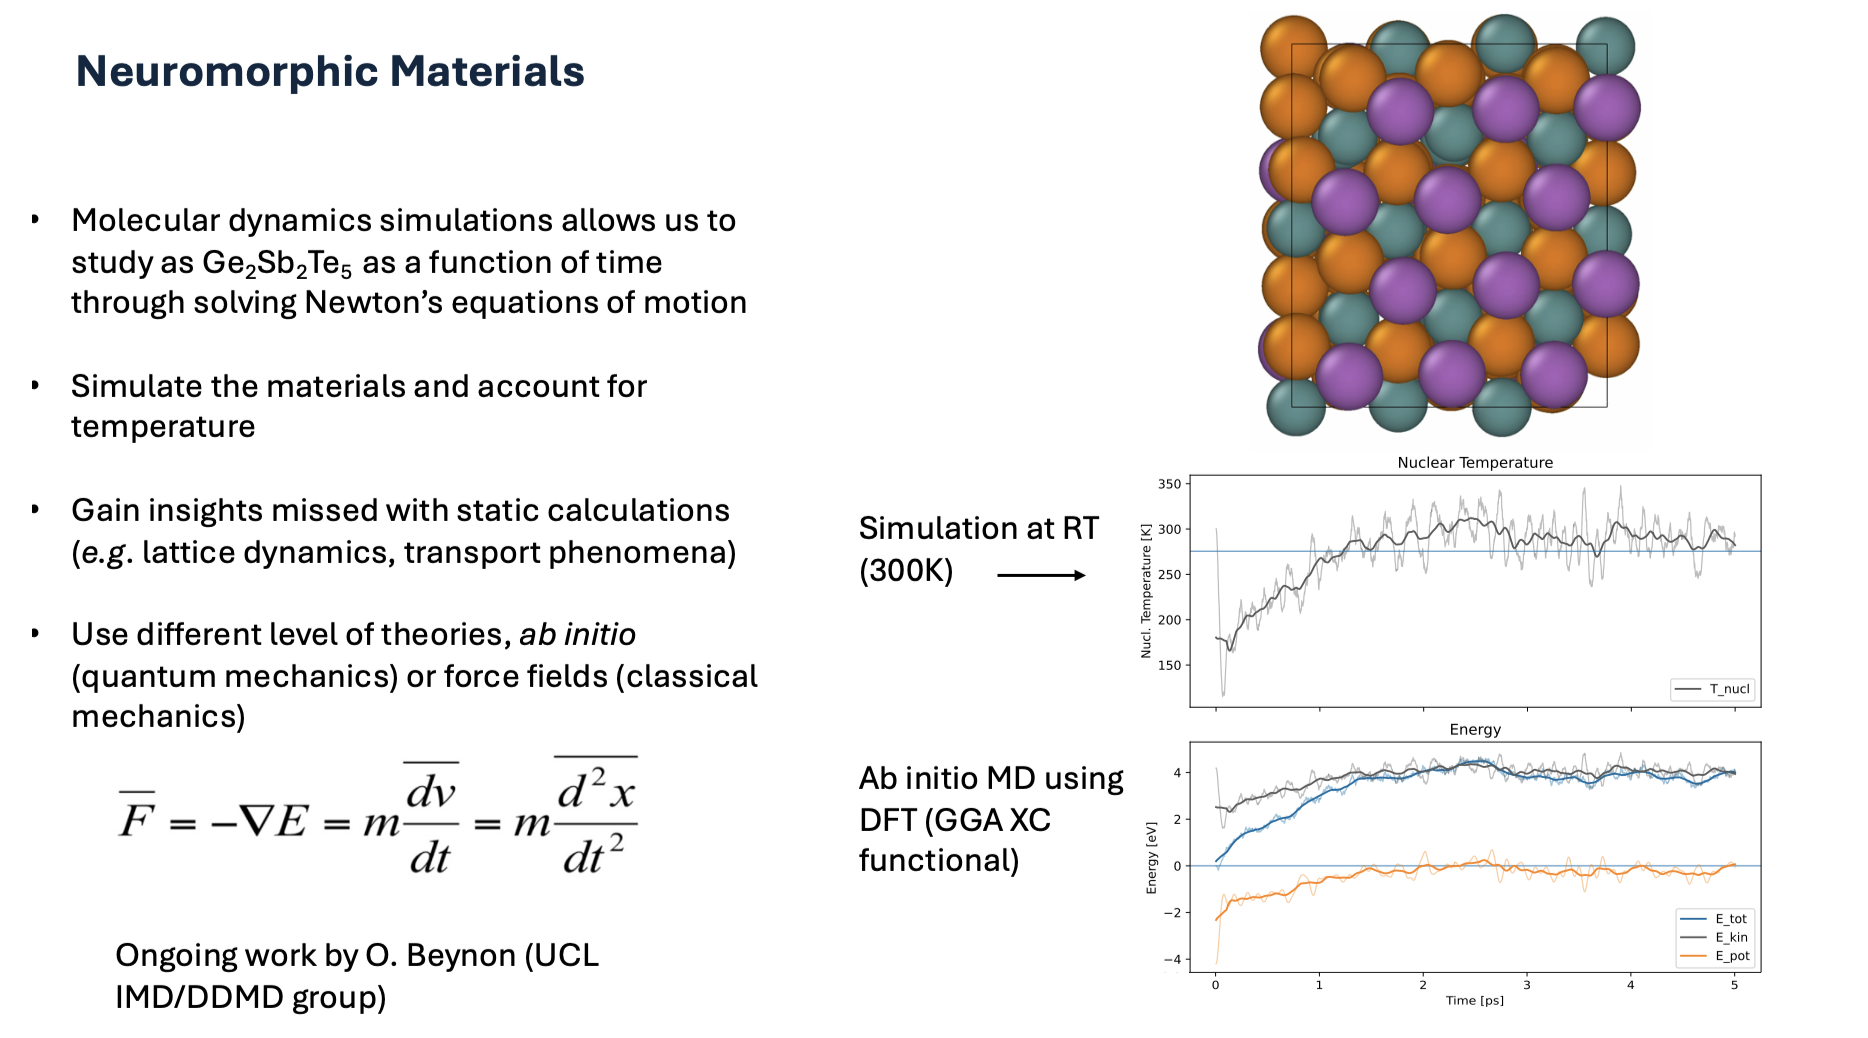
\includegraphics[width=0.75\textwidth]{media/gst_md.png}
\end{frame}




\begin{frame}{Neuromorphic Materials Layout}
  \begin{columns}[T] % Align all columns at the top

    % Left column: one tall image
    \begin{column}{0.33\textwidth}
      \centering
      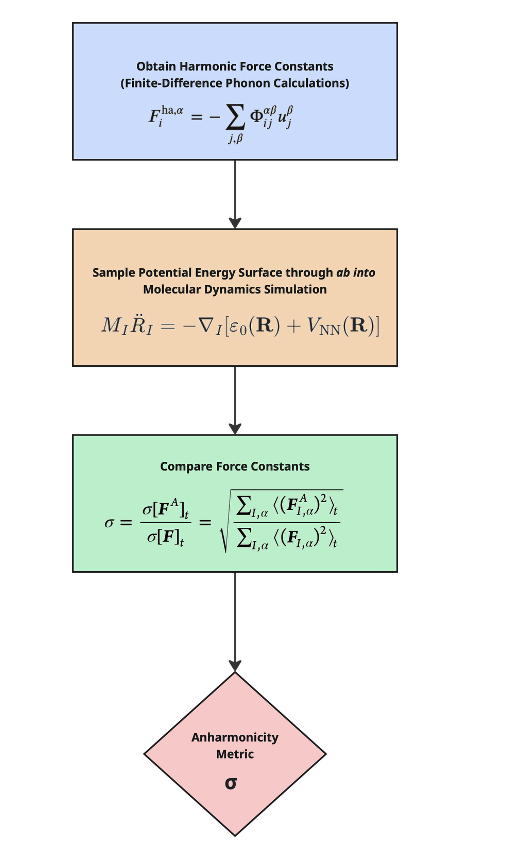
\includegraphics[height=0.7\textheight]{media/anharmonic_pipeline.png}
    \end{column}

    % Middle column: two stacked images
    \begin{column}{0.33\textwidth}
      \begin{minipage}[t]{\linewidth}
        \centering
        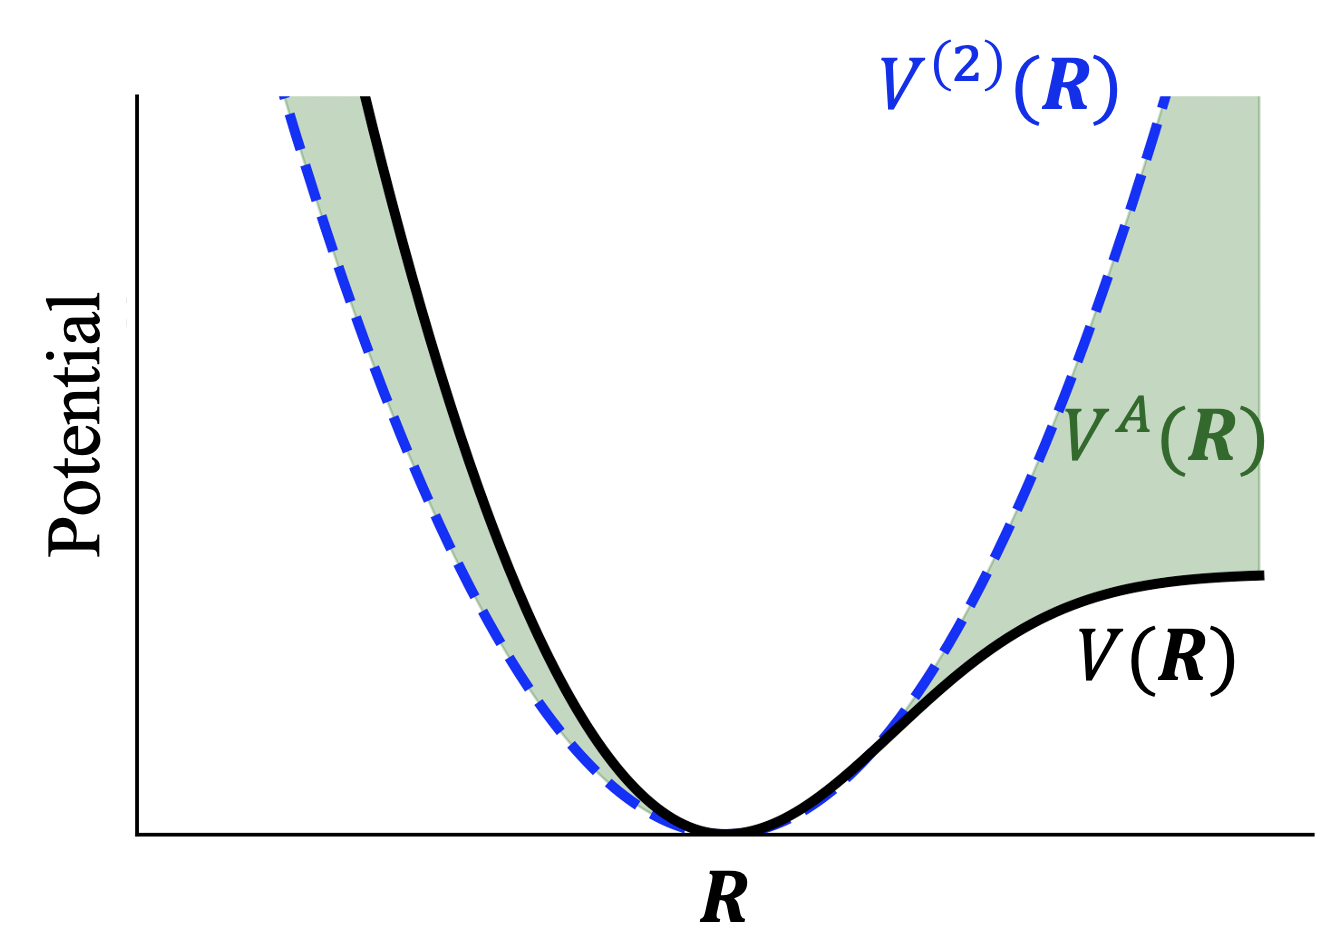
\includegraphics[width=0.6\textwidth]{media/harmonic.png}\\[1ex]
        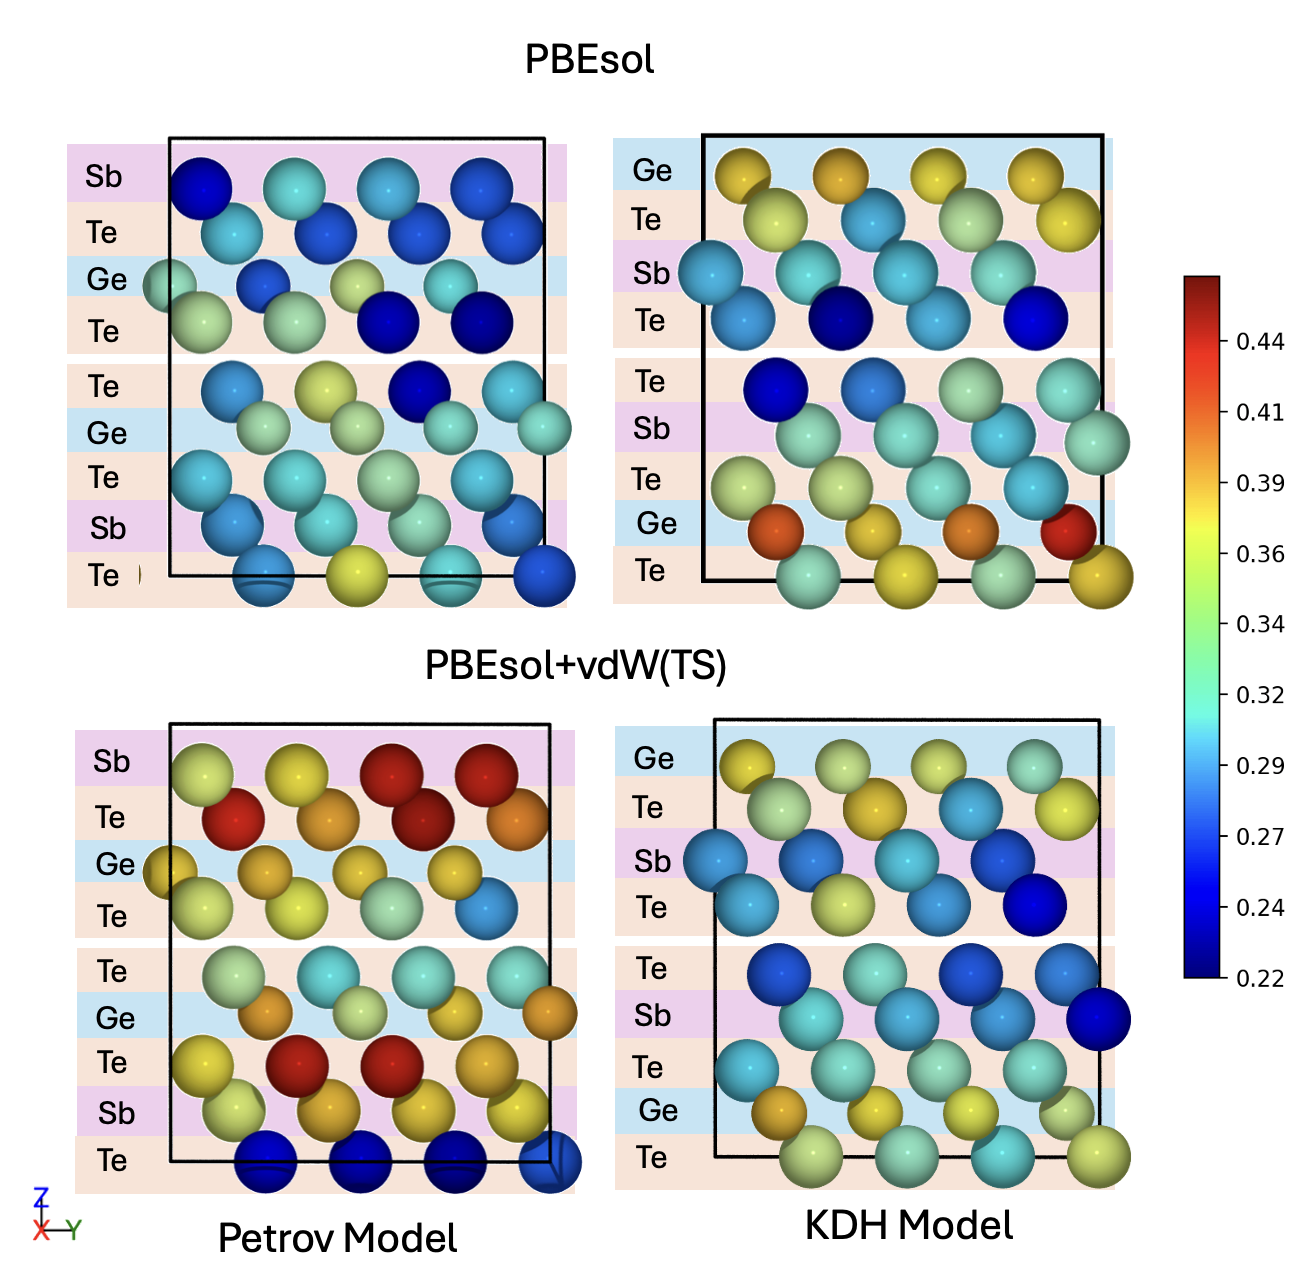
\includegraphics[width=0.6\textwidth]{media/pbesol_gst.png}
      \end{minipage}
    \end{column}

    % Right column: text block
    \begin{column}{0.33\textwidth}
      \small
      \begin{itemize}
        \item Anharmonic effects are important!
        \item (Owain, Hashibon, in preparation, 2025)
      \end{itemize}
    \end{column}

  \end{columns}
\end{frame}

%%%%%%%%%%%%%%%%%%%%%%%%%%%%%%%%%%%%%%%%%%%%%5

\begin{frame}{Data-Driven Materials Science}
    Leverage data to extract knowledge, rather than relying mainly on traditional theory or physics-based modelsi or empirical knowledge.

    \vspace{1em}
    \begin{itemize}
        \item Data becomes a key driver of discovery and innovation.
        \item This approach contrasts with classical methods rooted in {mathematics and physical theory}.
        \item The shift: \textit{From equations to correlations, from models to patterns}.
        \item \textit{Data is not just a result any more but it is the {\bf engine of knowledge}}
        \item But we still and in addition,  look at {materials modelling}, where simulations and computational methods generate valuable data.
    \end{itemize}

    \vspace{1em}
\end{frame}


\begin{frame}{The role of Digitalisation in Data-Driven Materials Science}

    \vspace{1em}
    \begin{itemize}
        \item \textbf{Data-Driven Systems} shift the paradigm from theory-based to information-based discovery.
        \item \textbf{Materials Modelling} generates data that fuels knowledge extraction.
        \item This approach supports the concept of a \textbf{Digital Twin}—a virtual replica of a material or process.
        \item We move from physical experimentation to \textit{computational exploration}.
    \end{itemize}

    \textbf{Digitalisation} of materials enables us to process and understand materials without direct physical interaction, working instead with their digital representations --> Digital Models.
    \vspace{1em}
    \textit{Digitalisation is not just a tool—it’s a transformation of how we do materials science.}
\end{frame}



\begin{frame}{Digitalisation}
    \begin{columns}
        \column{0.6\textwidth}
        Dictionary definition:\textbf{digitalization} | (digitalisation)\\
        \textbf{noun} [mass noun]\\
        adaptation of a system, process, etc. to be operated with the use of computers and the internet: \\
        \textit{digitalization allowed companies to sell goods without a physical presence} \\

        \vspace{1em}
        \textcolor{purple}{to Process “material” without their physical presence = working with the information about the material.}

        \vspace{0.5em}
        This is the so called \textcolor{red}{\textbf{Digital Twin}}

        {\tiny  \href{https://www.3ds.com/products/delmia/virtual-twin-manufacturing}{image credit: 3ds}}
        \column{0.4\textwidth}
        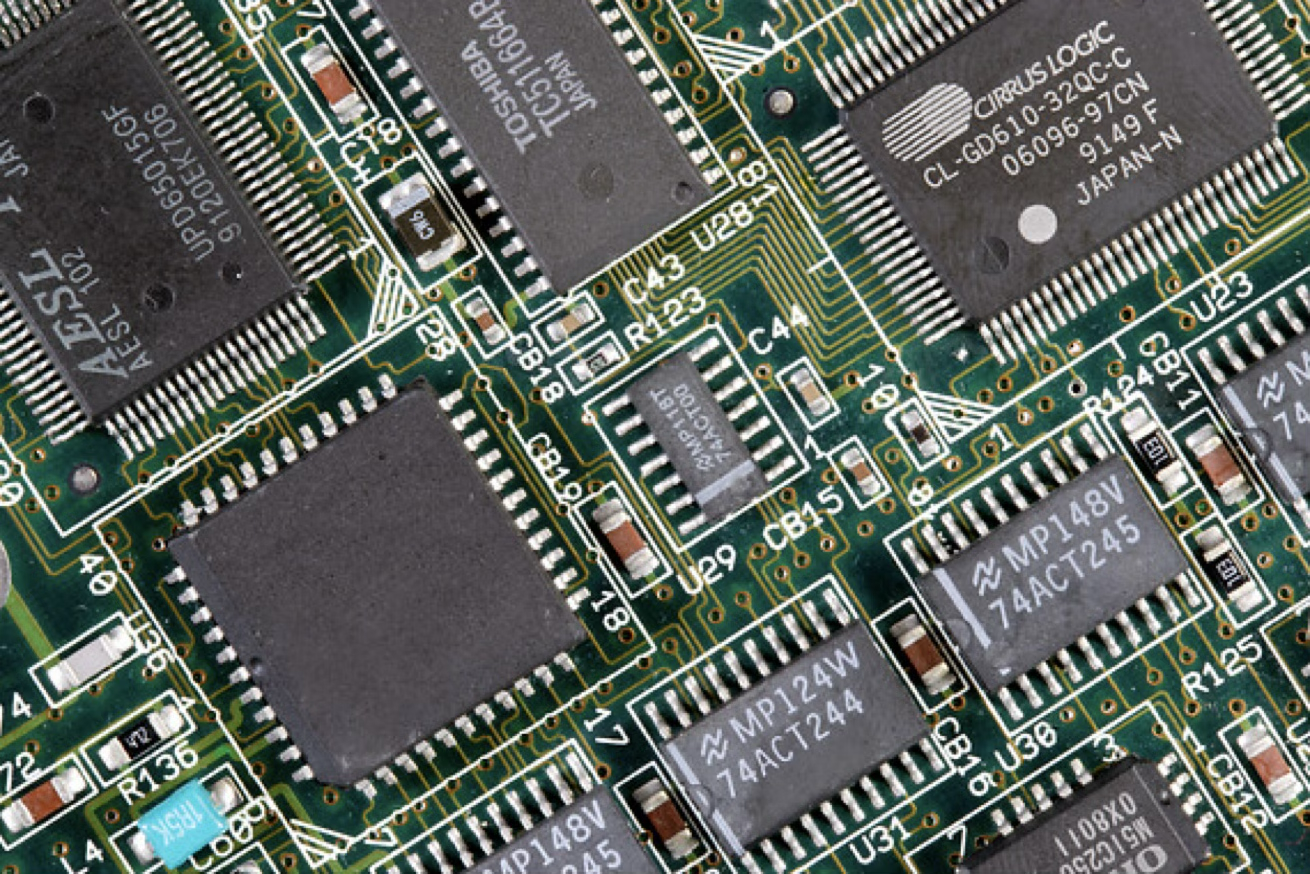
\includegraphics[width=\linewidth]{media/circuit.png}\\[0.5em]
        
\includegraphics[width=\linewidth]{media/digital_twin.png}
    \end{columns}
\end{frame}


\begin{frame}{Digitalisation vs Digitisation}
    \begin{center}
        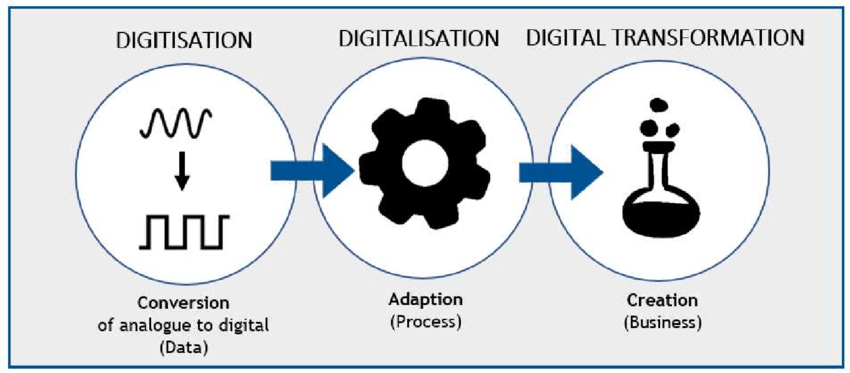
\includegraphics[width=0.4\linewidth]{media/digi_digi.png}
        {\tiny Buman and Mark}
    \end{center}

    \vspace{1em}
    \begin{itemize}
        \item \textbf{Digitisation}: Conversion of physical formats (e.g., paper, stone) into digital media (e.g., disk, memory).
        \item \textbf{Digitalisation}: Goes beyond digitisationr, it's about transforming processes and systems using digital technologies
        \item Raises the question: \textit{What does digitalisation mean for materials science?}
    \end{itemize}
\end{frame}



\begin{frame}{{\it Traditional} Materials Discovery}
  \begin{columns}
        \column{0.5\textwidth}
    \begin{itemize}
        \item Use experiments and  empirical knowledge to suggest materials or optimise existing ones
        \item Focuses on a particular material, and sometimes also a process (though often neglected)
        \item Example: \textit{"What are the mechanisms of Li conductance in $M_3N$ ($M = \text{Nb, Ta}$)?"}
        \item Test and repeat: Generate small, targeted number of experiments and simulations
        \item (Very) Small amount of data
    \end{itemize}

        \column{0.5\textwidth}
    \vspace{1em}
    \begin{center}
        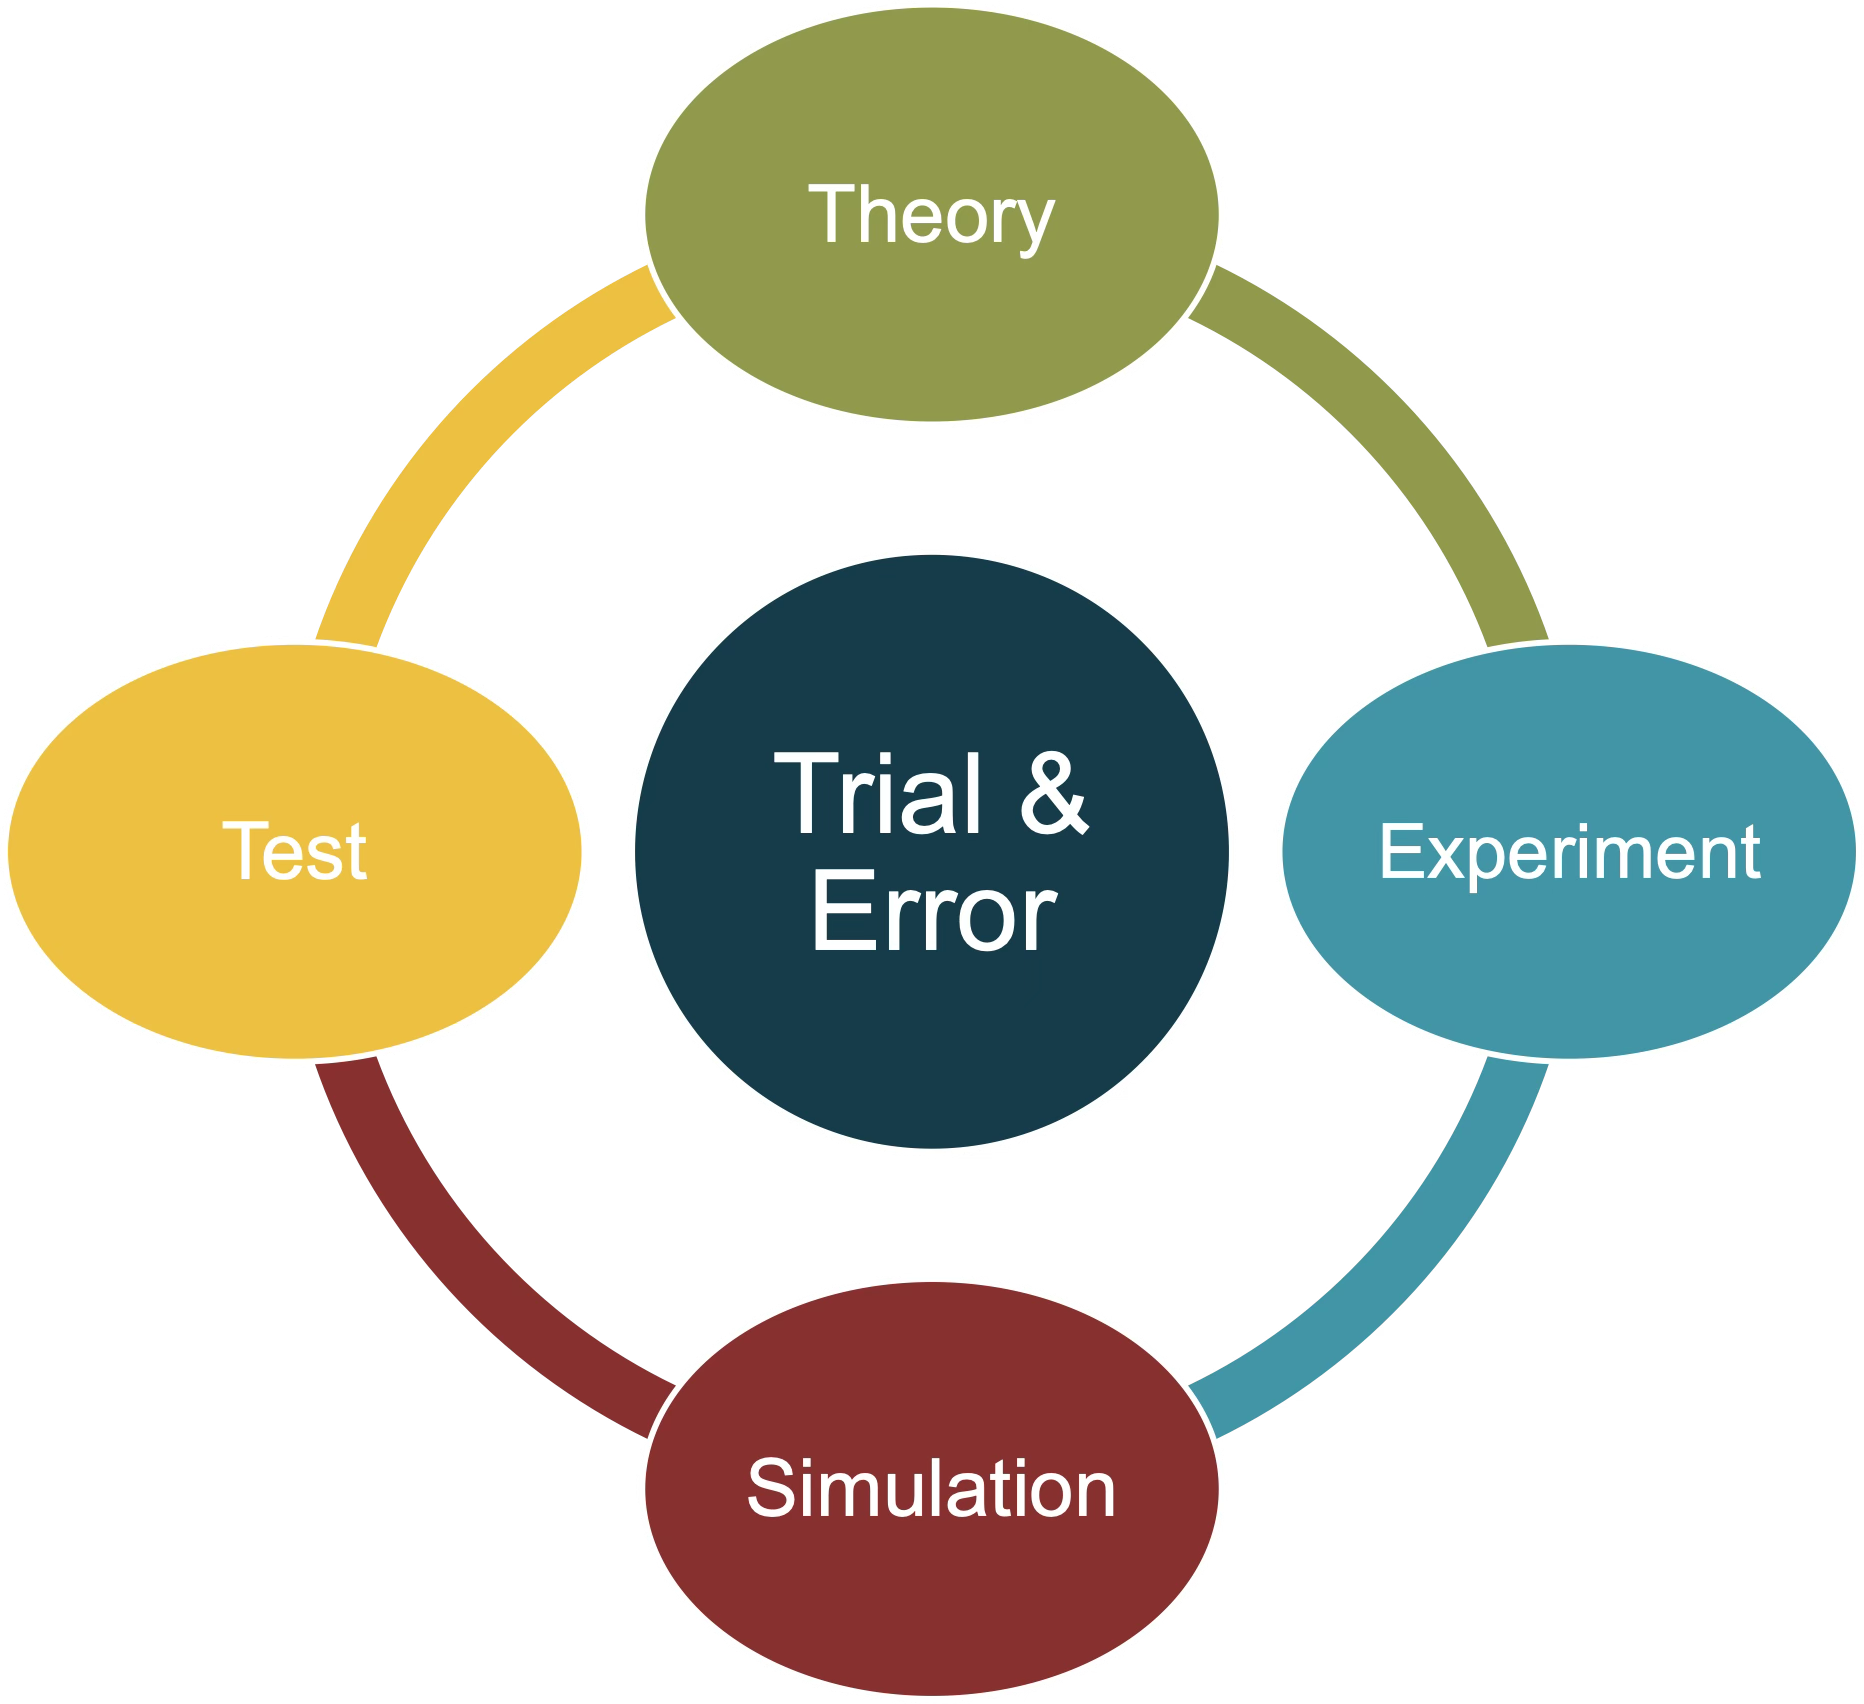
\includegraphics[width=0.75\linewidth]{media/traditional_science.png}
    \end{center}
  \end{columns}
\end{frame}

\begin{frame}{A Typical Example...}
  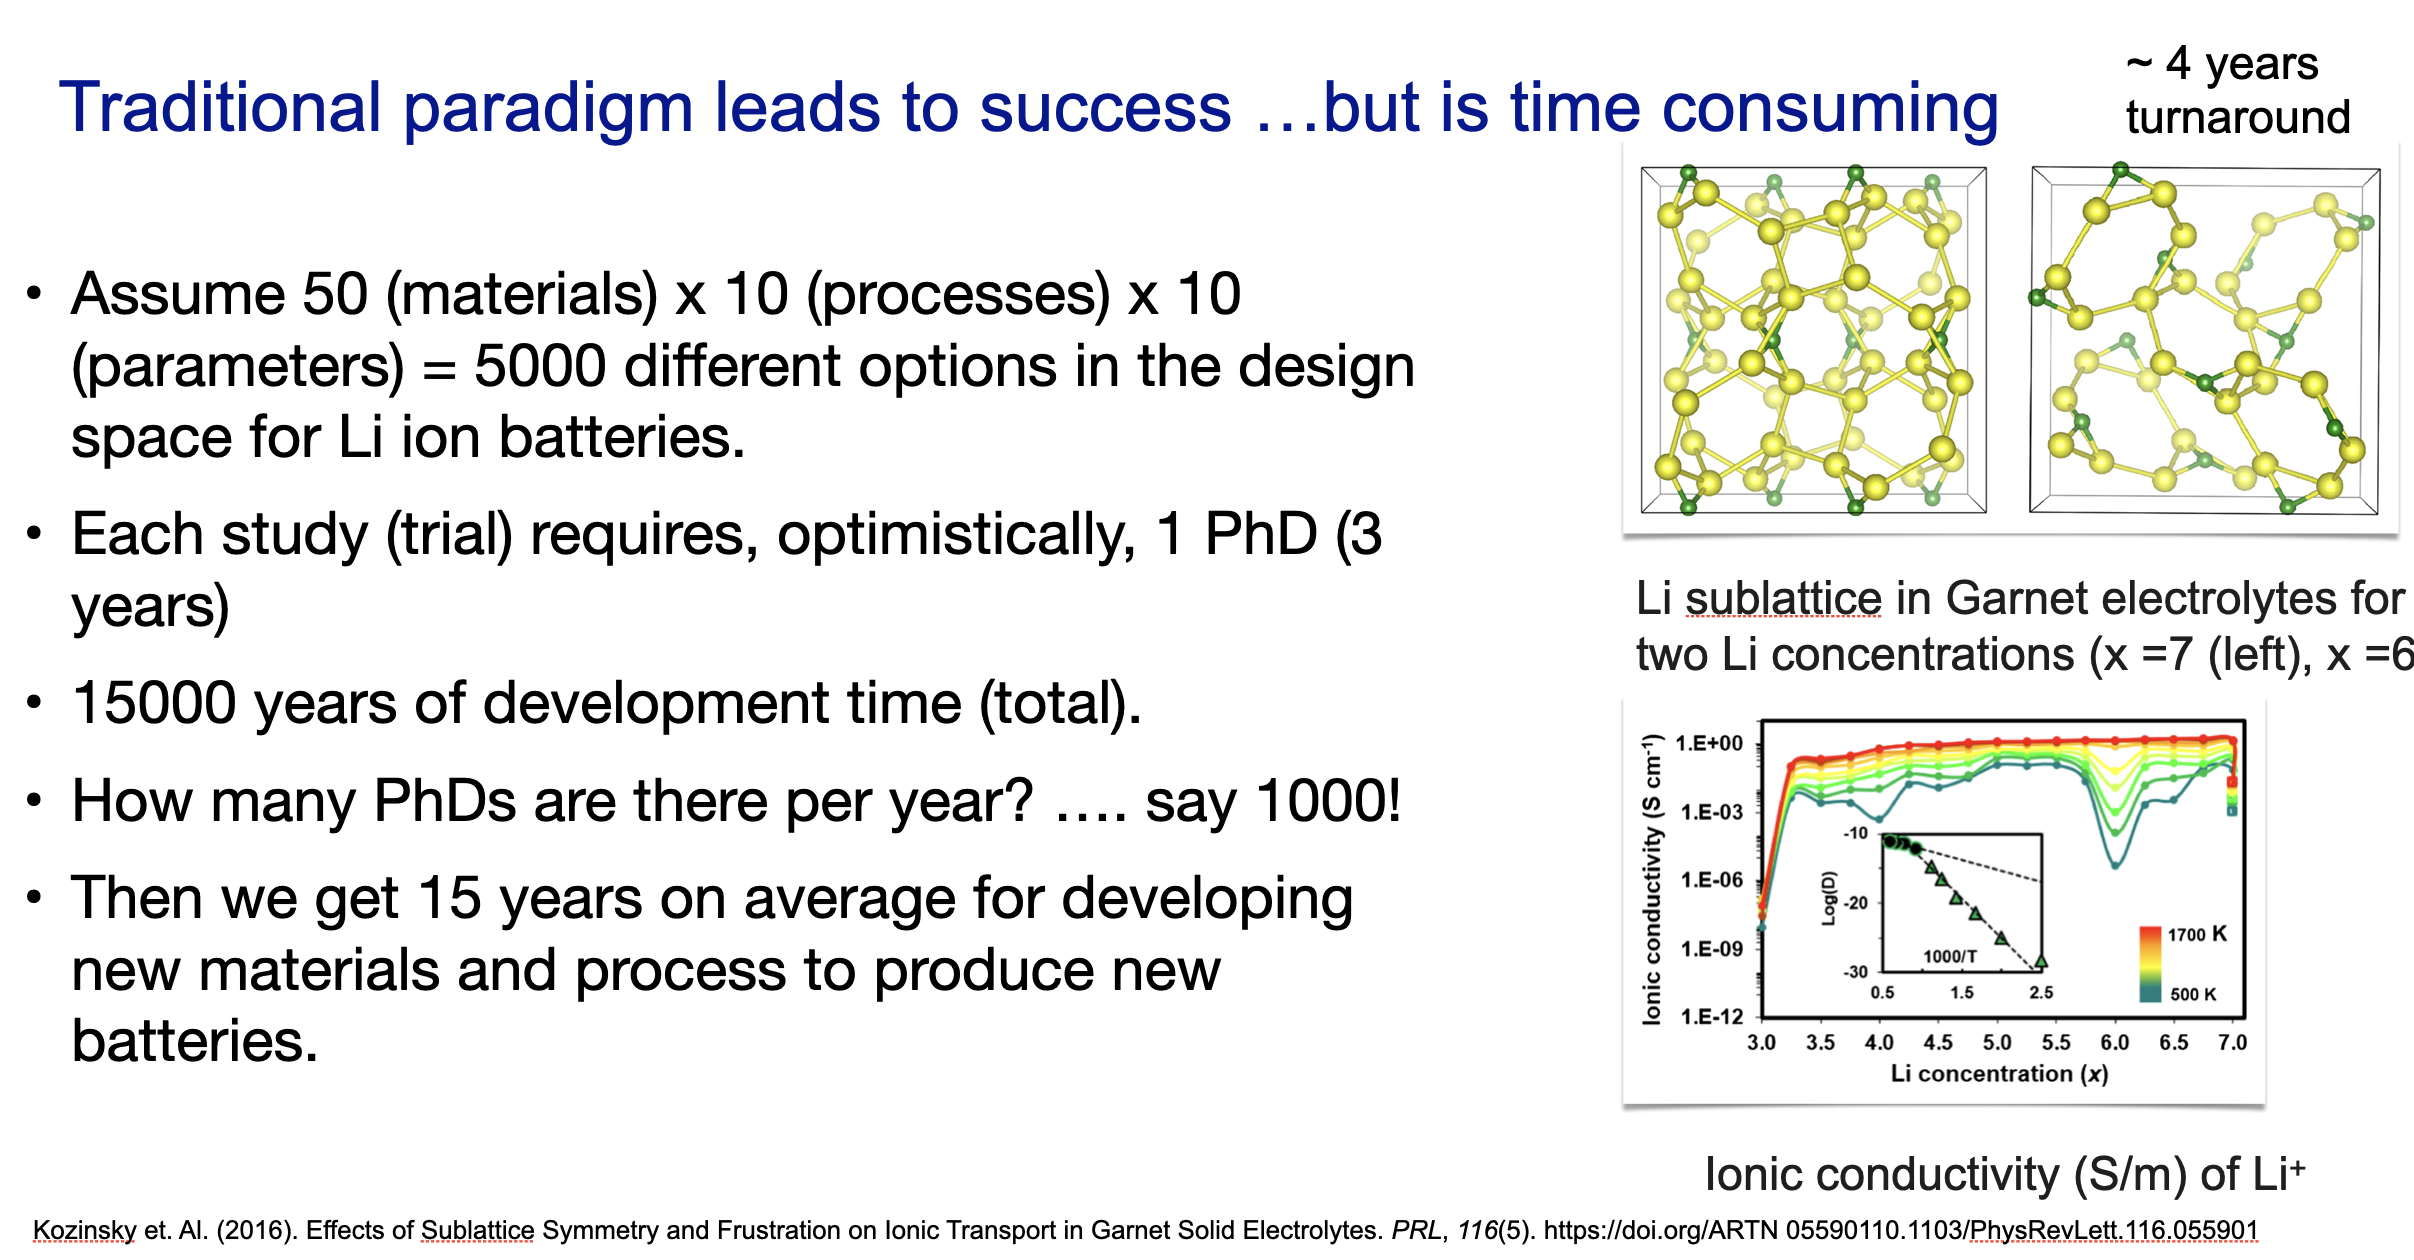
\includegraphics[width=0.75\textwidth]{media/garnet_time.png}
\end{frame}

\begin{frame}{The actual history of Li-ion battery}
  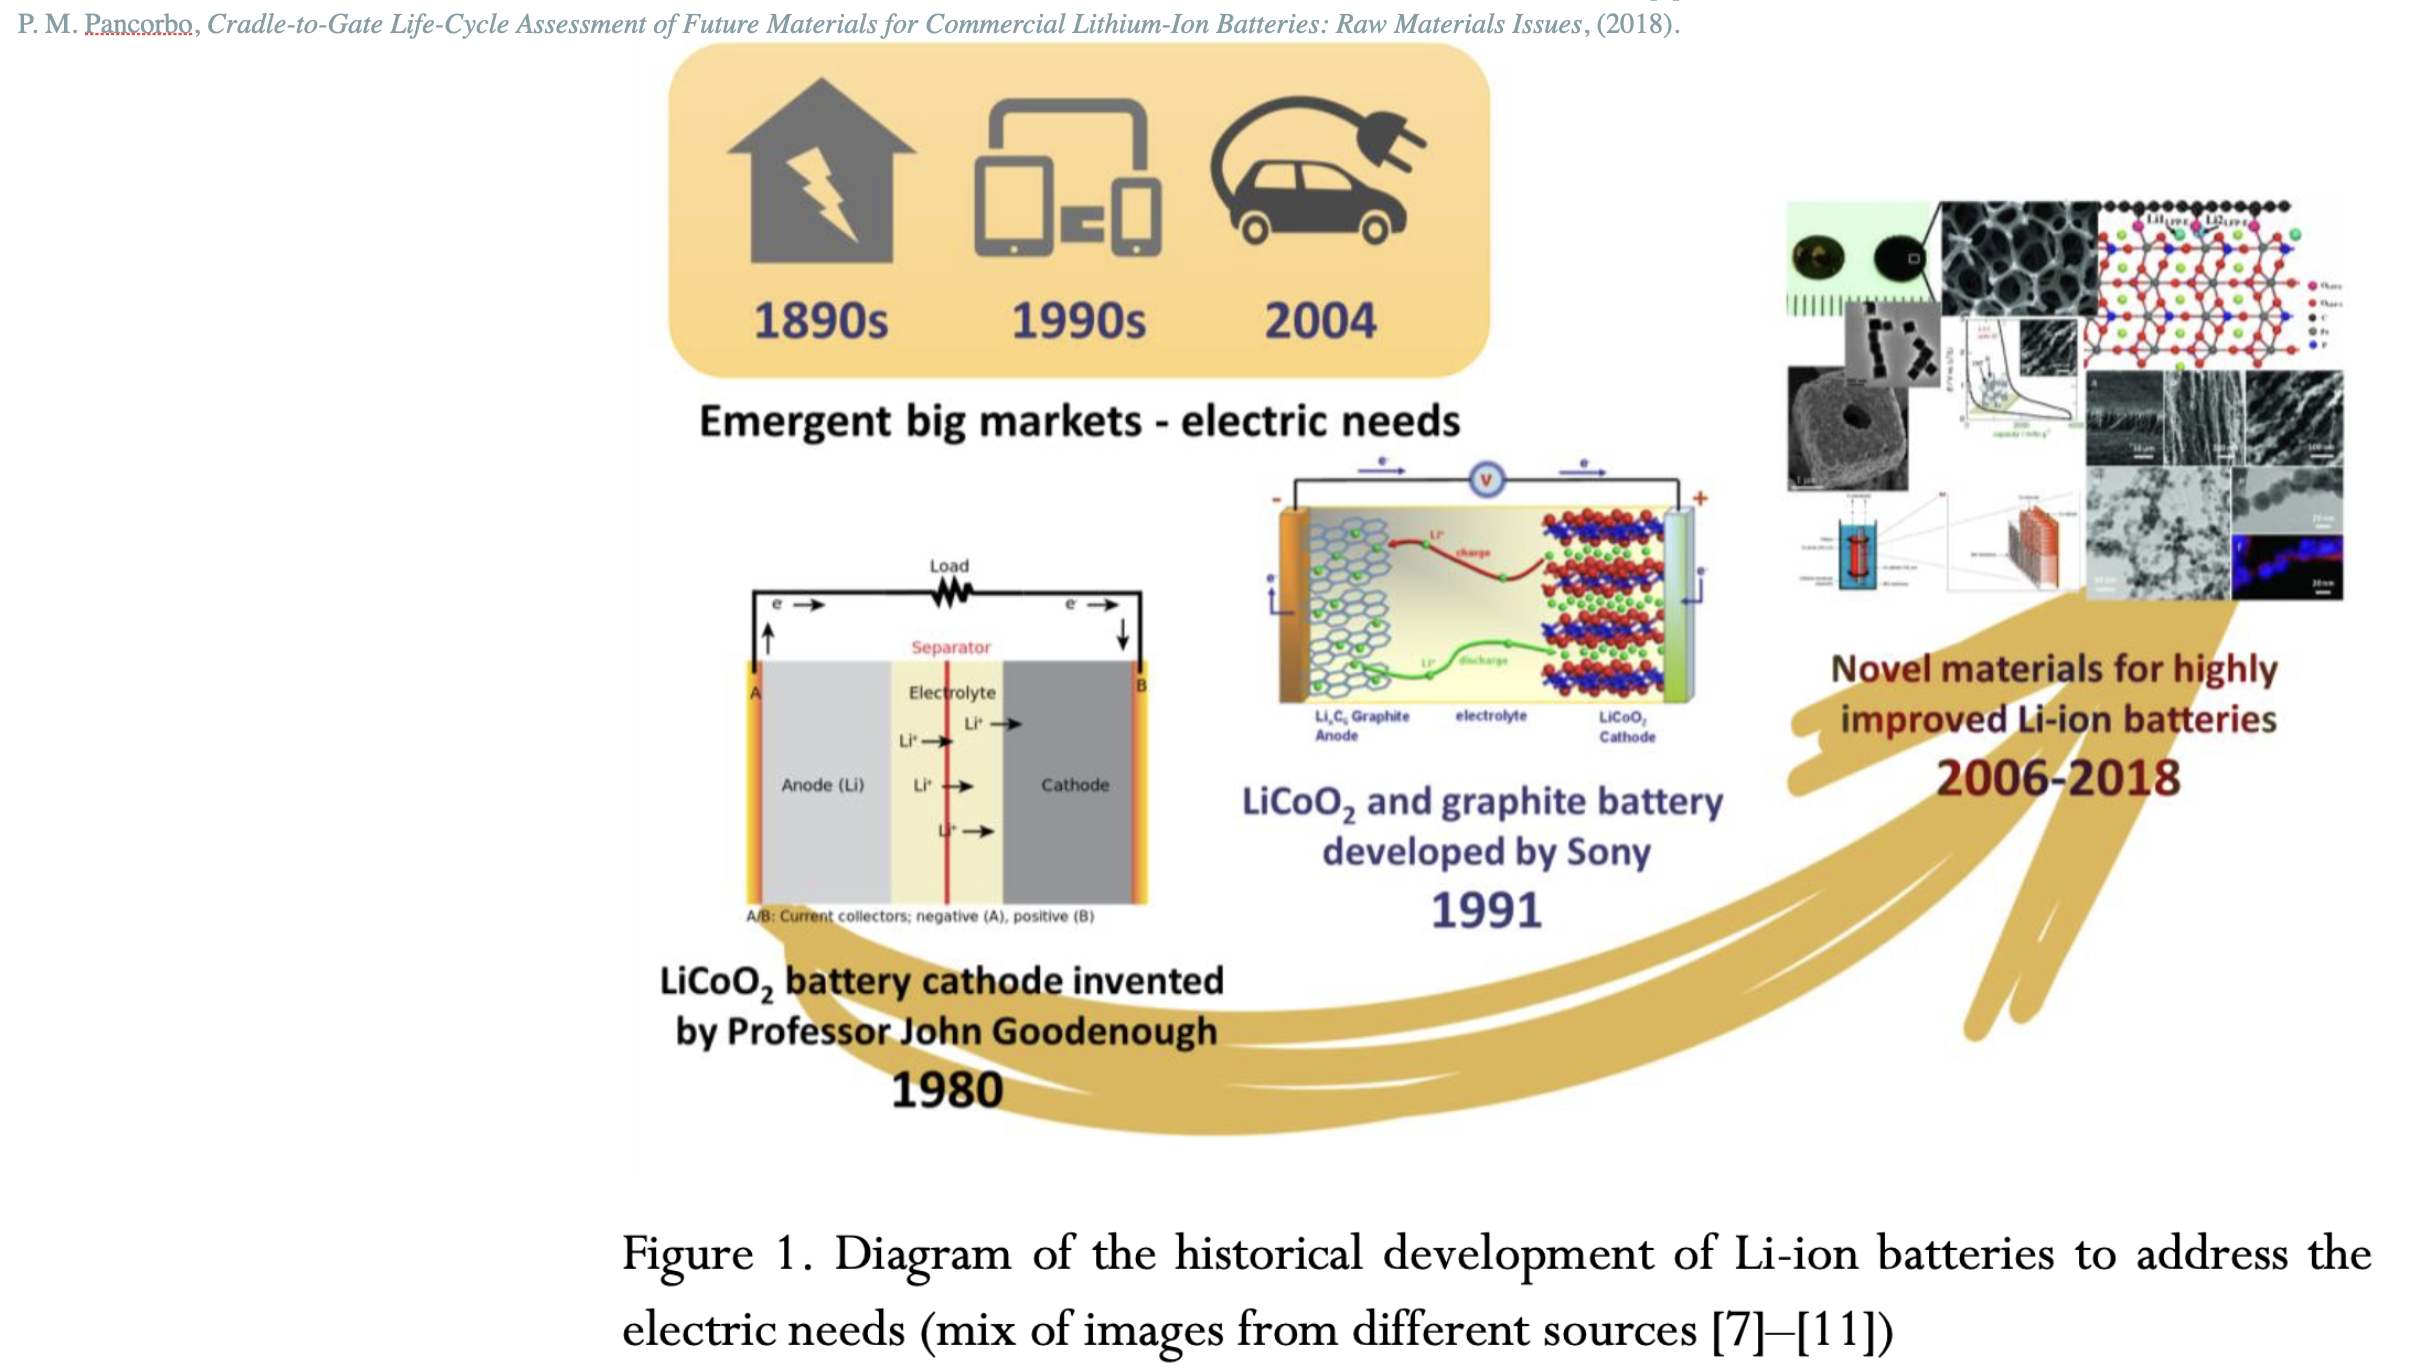
\includegraphics[width=0.75\textwidth]{media/battery_history.png}
\end{frame}

\begin{frame}{Did you know that...}
  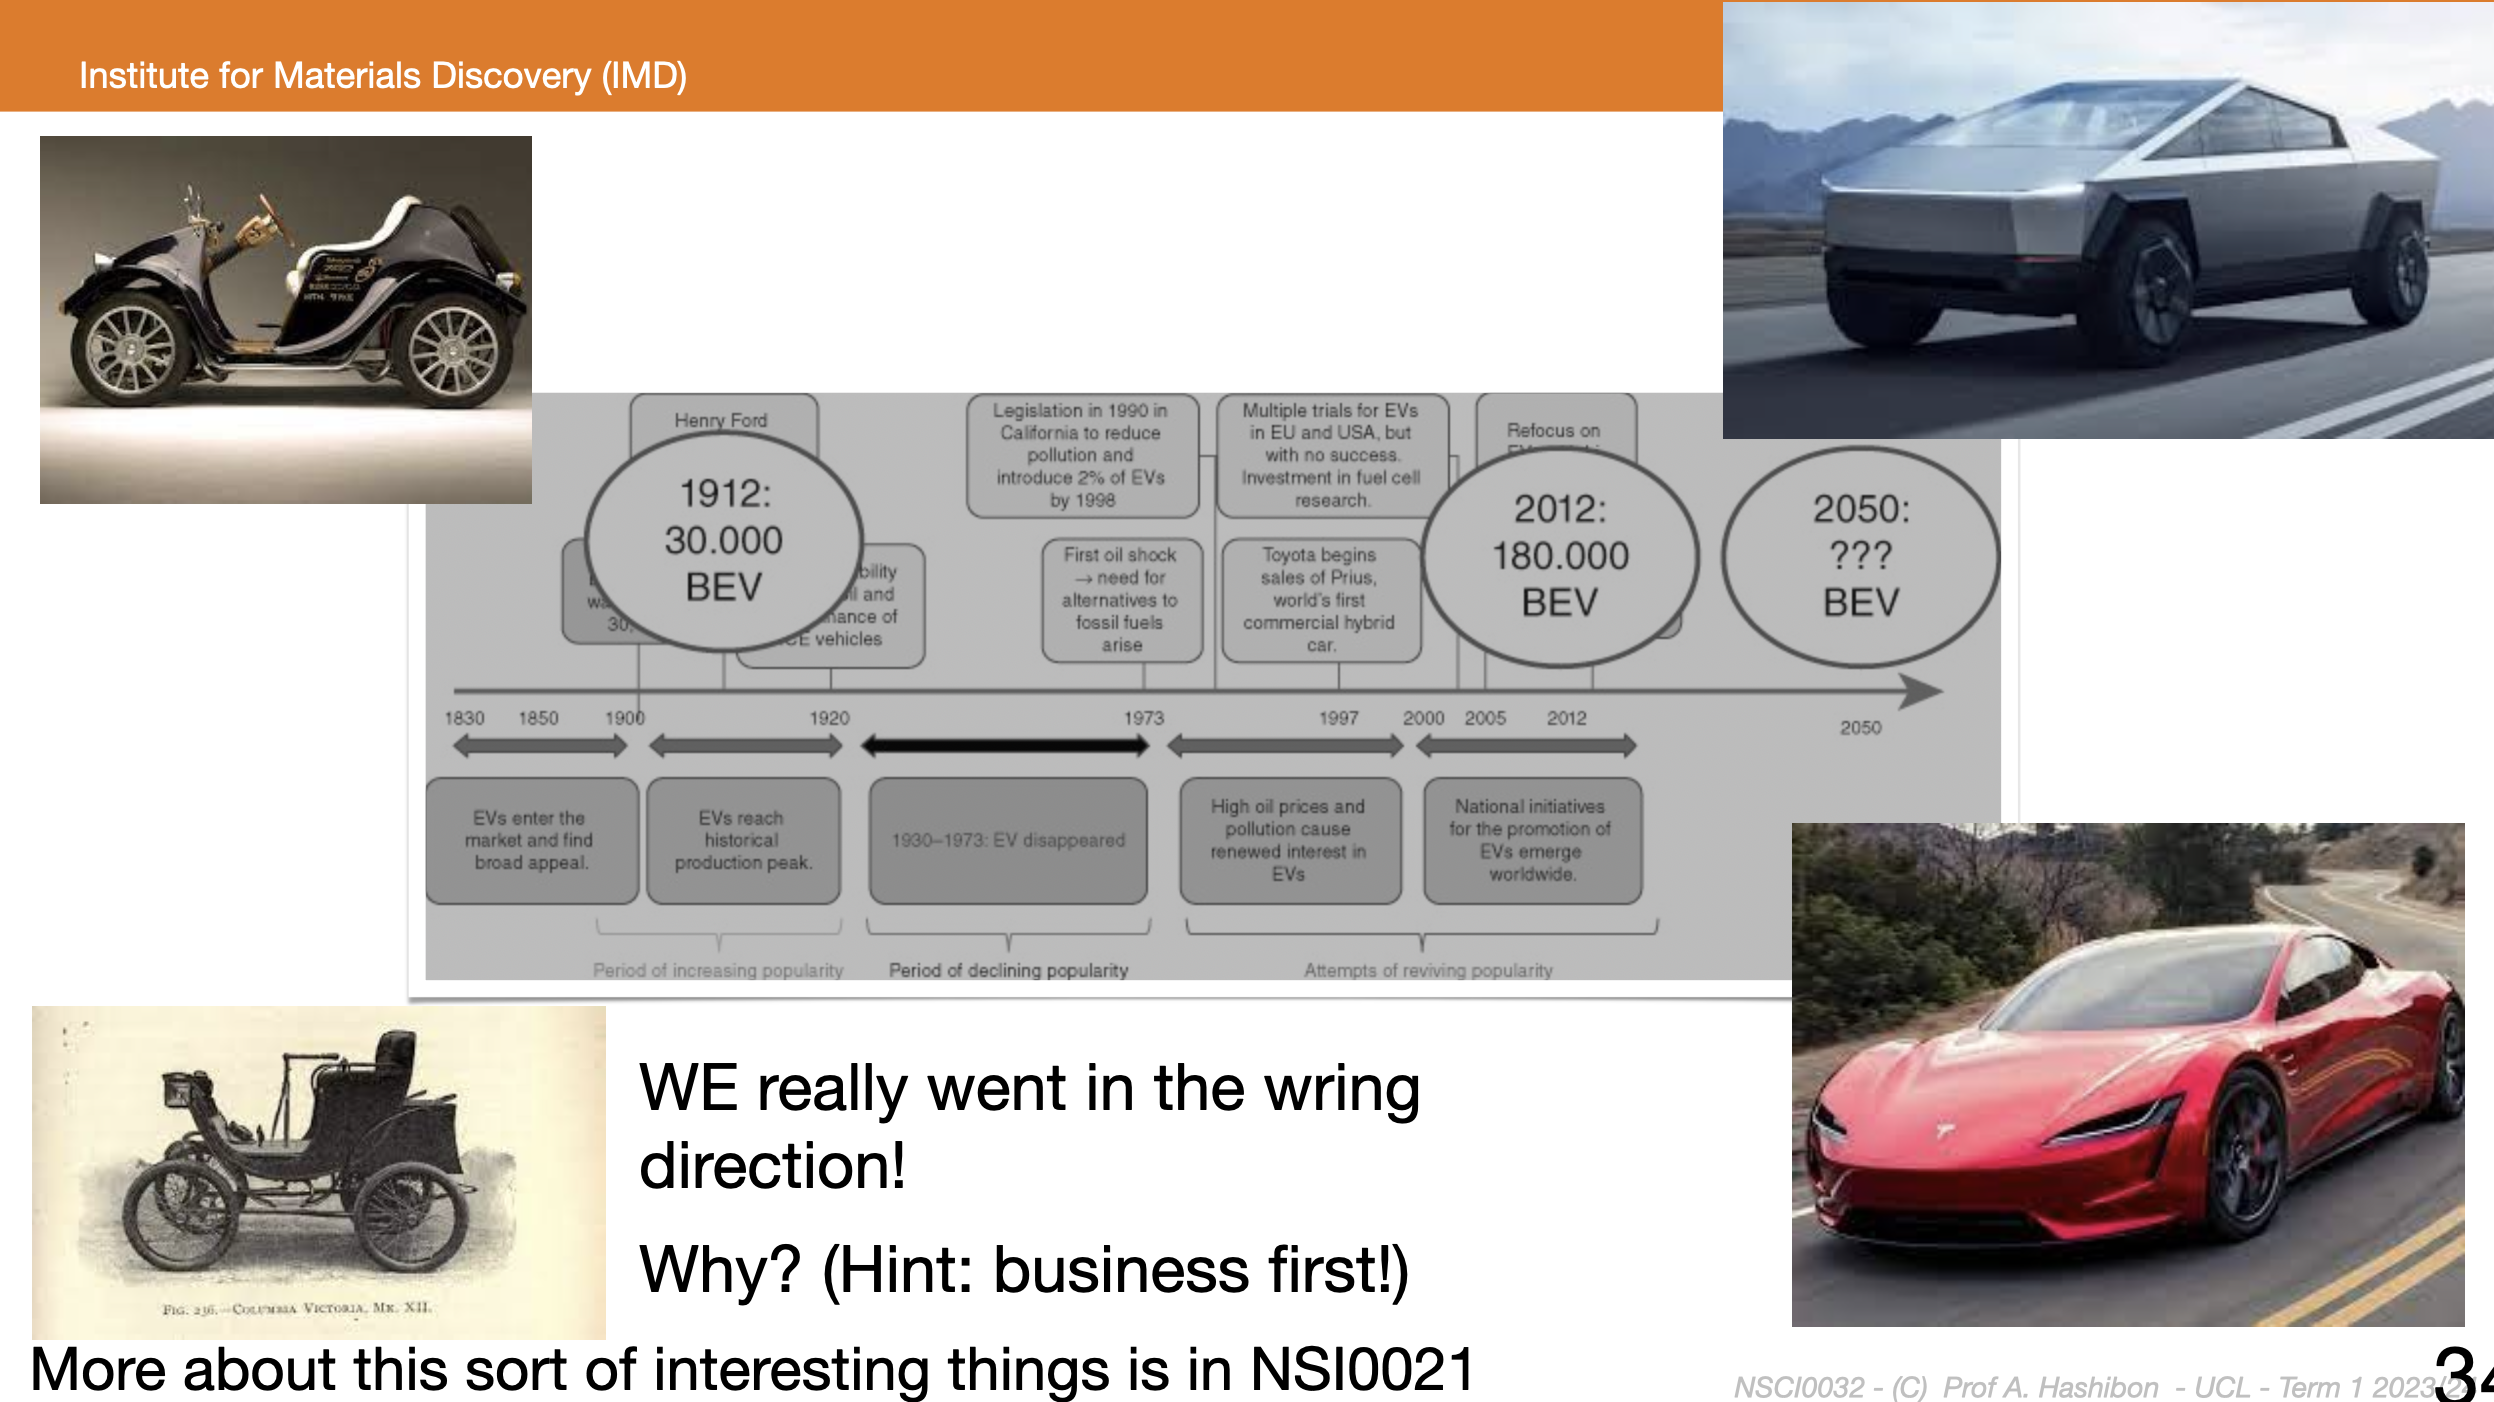
\includegraphics[width=0.75\textwidth]{media/old_cars.png}
\end{frame}

\begin{frame}{\it Self-Starting Cadillac, 1912}
  \begin{columns}
    \column{0.5\textwidth}
    From \textit{Toronto Sunday World}, Feb. 18, 1912.\\
    The release of the first practical electric self-starter on the 1912 Cadillacs was a major event.\\
    Contemporary reports said that the new technology was “of more interest to motorists than any other.”\\
    The self-starter also established the need for electrical systems on future gasoline cars, creating a much more lucrative industry for battery companies than for powering electrics.

    \column{0.5\textwidth}
    \vspace{1em}
    \begin{center}
      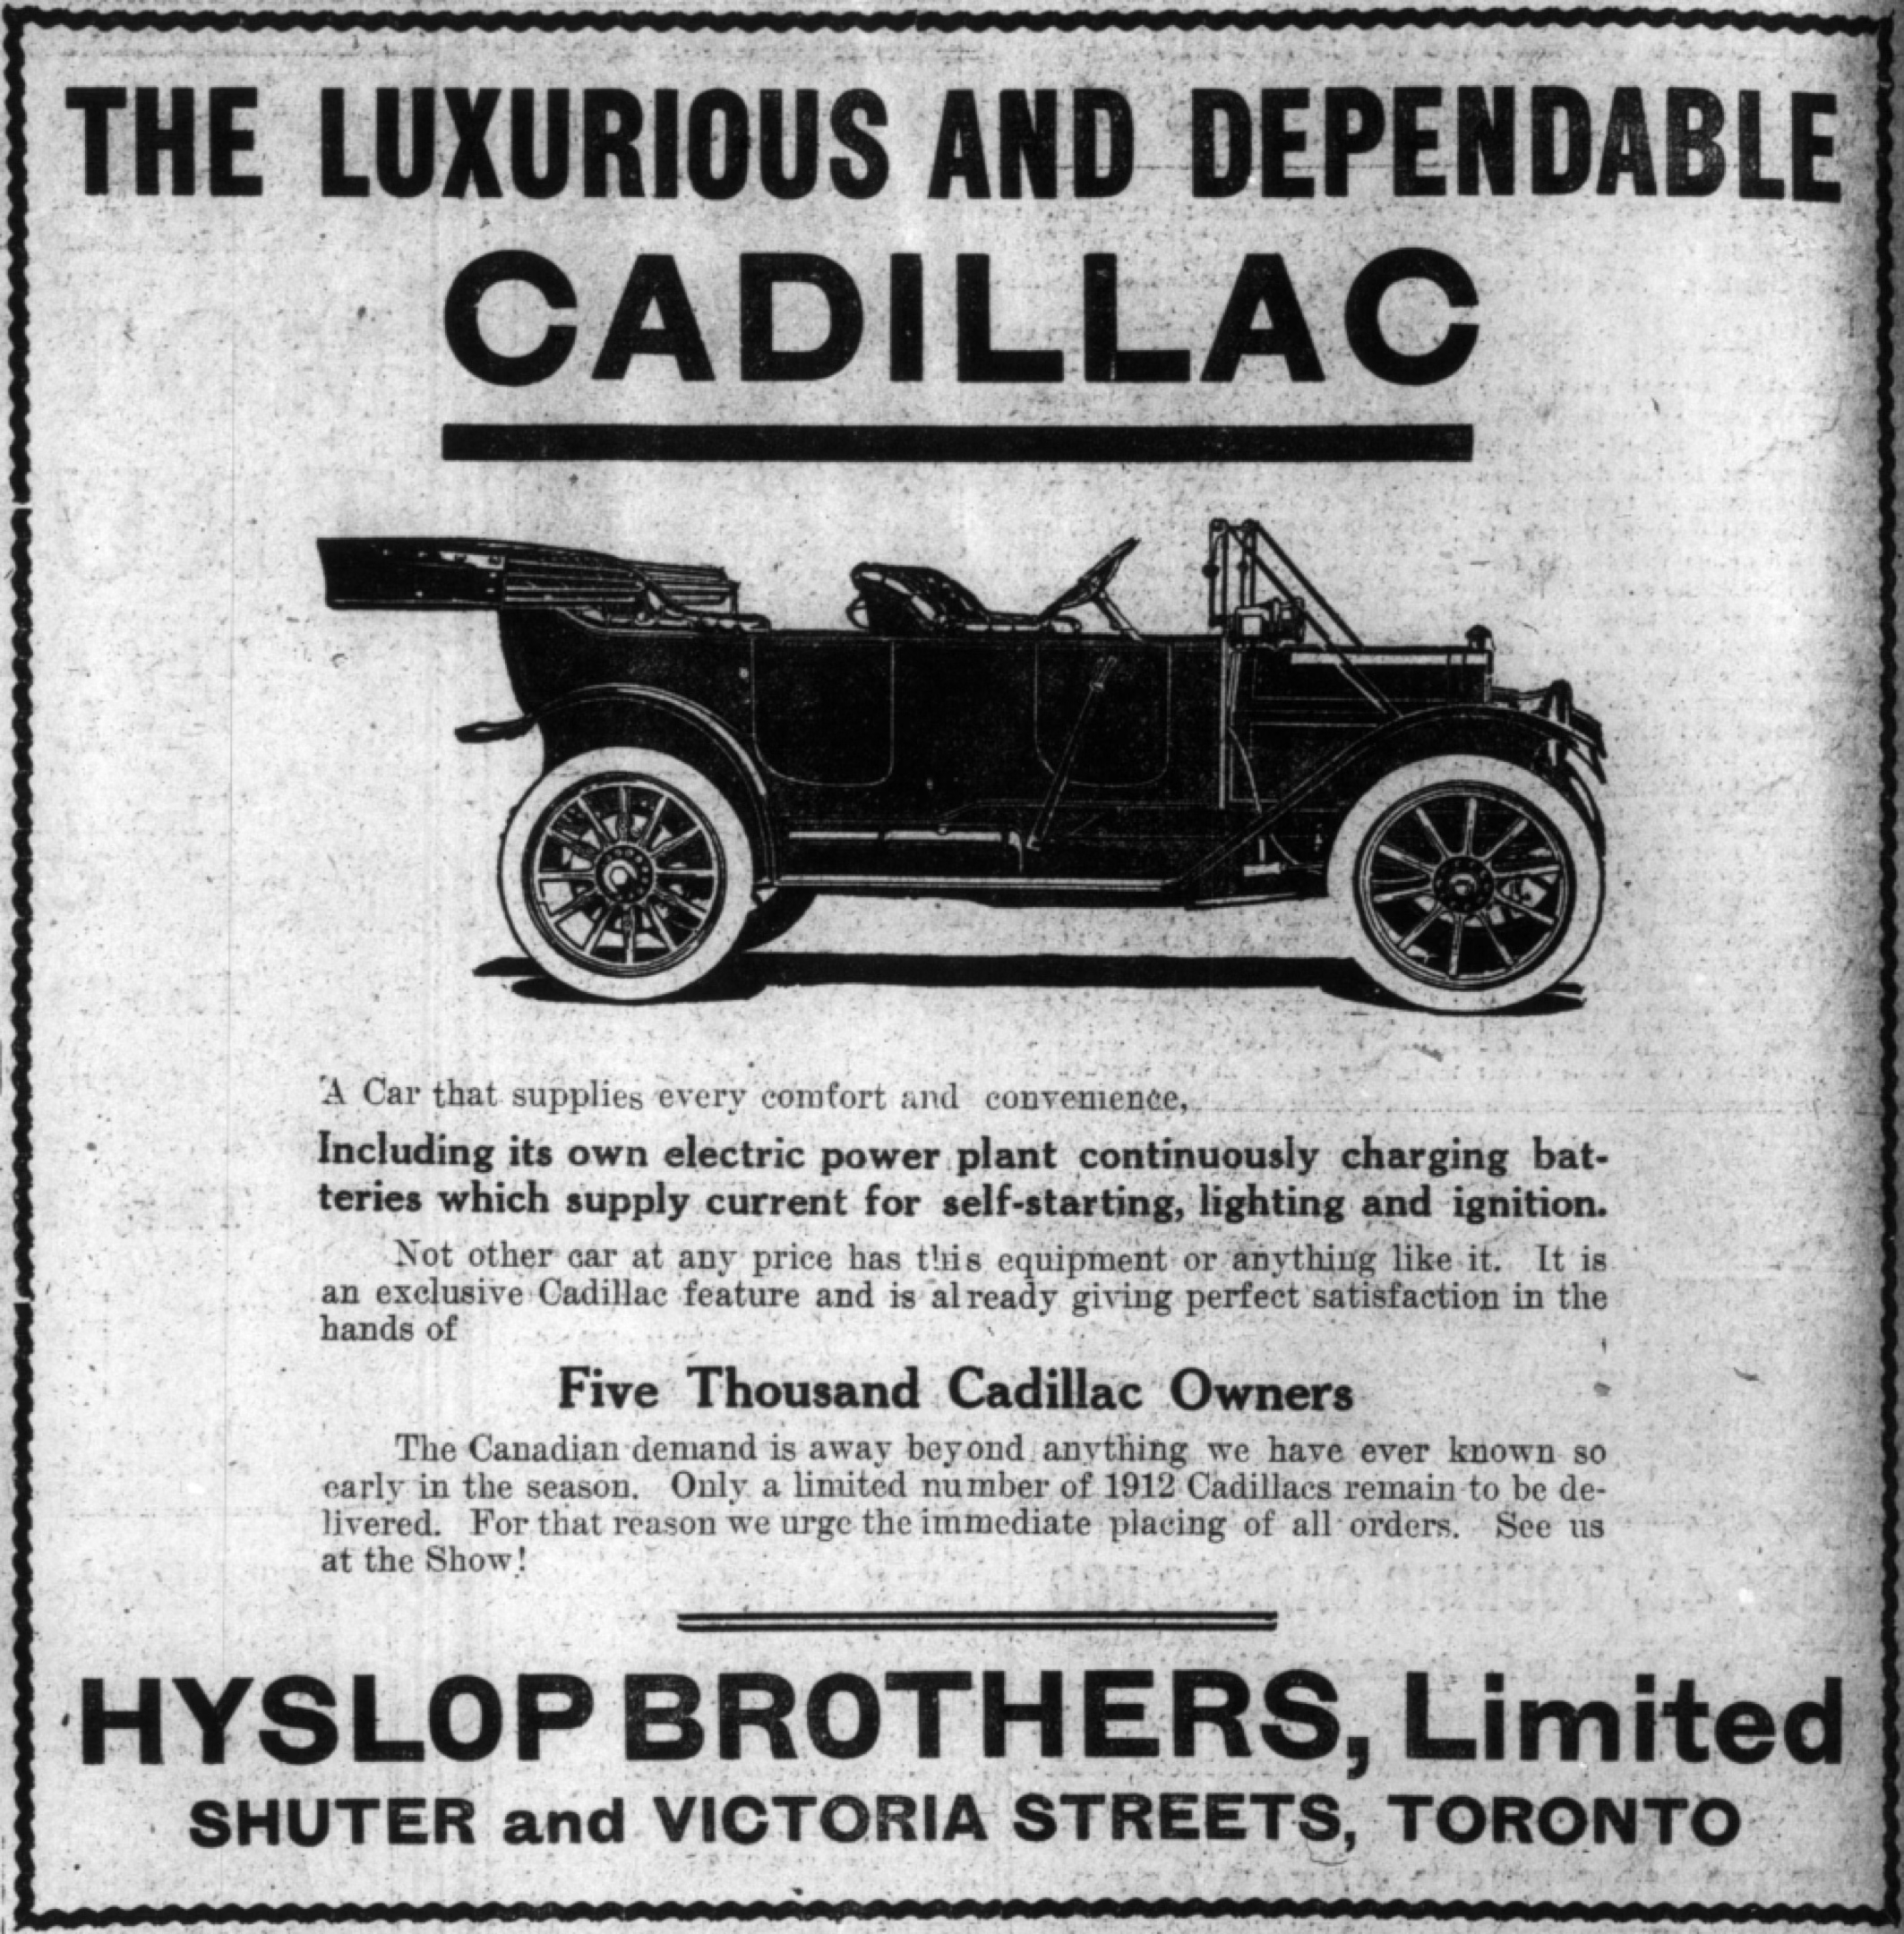
\includegraphics[width=0.75\linewidth]{media/caddilac.png} % Correct spelling?
    \end{center}
  \end{columns}
\end{frame}

%%%%%%%%%%%%
%%%%%%%%%%%%
\end{document}
